%!TEX root = ../thesis.tex

\chapter{The LHC and the CMS detector}
\label{c:detector}
\ifpdf
    \graphicspath{{03_Detector/plots/}}
\else
    \graphicspath{{03_Detector/plots/EPS/}{03_Detector/plots/}}
\fi

\section{The Large Hadron Collider}
\label{s:LHC}

The LHC \autocite{LHC} is currently the largest and the most powerful particle accelerator ever built. It is installed
in the \SI{26.7}{\km} tunnel that was originally constructed for the LEP accelerator in the 1980s. The tunnel lies at a
depth of \SIrange{45}{170}{\metre} underground between the Jura mountain and Lake Geneva, being the main part of the
CERN accelerator complex.

The machine is designed to accelerate proton beams and provide collisions at a centre of mass energy of $\sqrt s =$
\SI{14}{\TeV}. Unlike particle-antiparticle colliders, the LHC requires two rings with opposite magnetic dipole fields
in order to maintain and collide two counter-rotating proton beams. Since the tunnel was originally designed for the
electron-positron LEP, it has an internal diameter of \SI{3.7}{\metre} which is not enough to install two separate
independent rings. Therefore, a twin-bore magnet design was adopted \autocite{Blewett}, which resulted in substantial
cost savings.

\begin{figure}[!htbp]
  \centering
  \leavevmode
  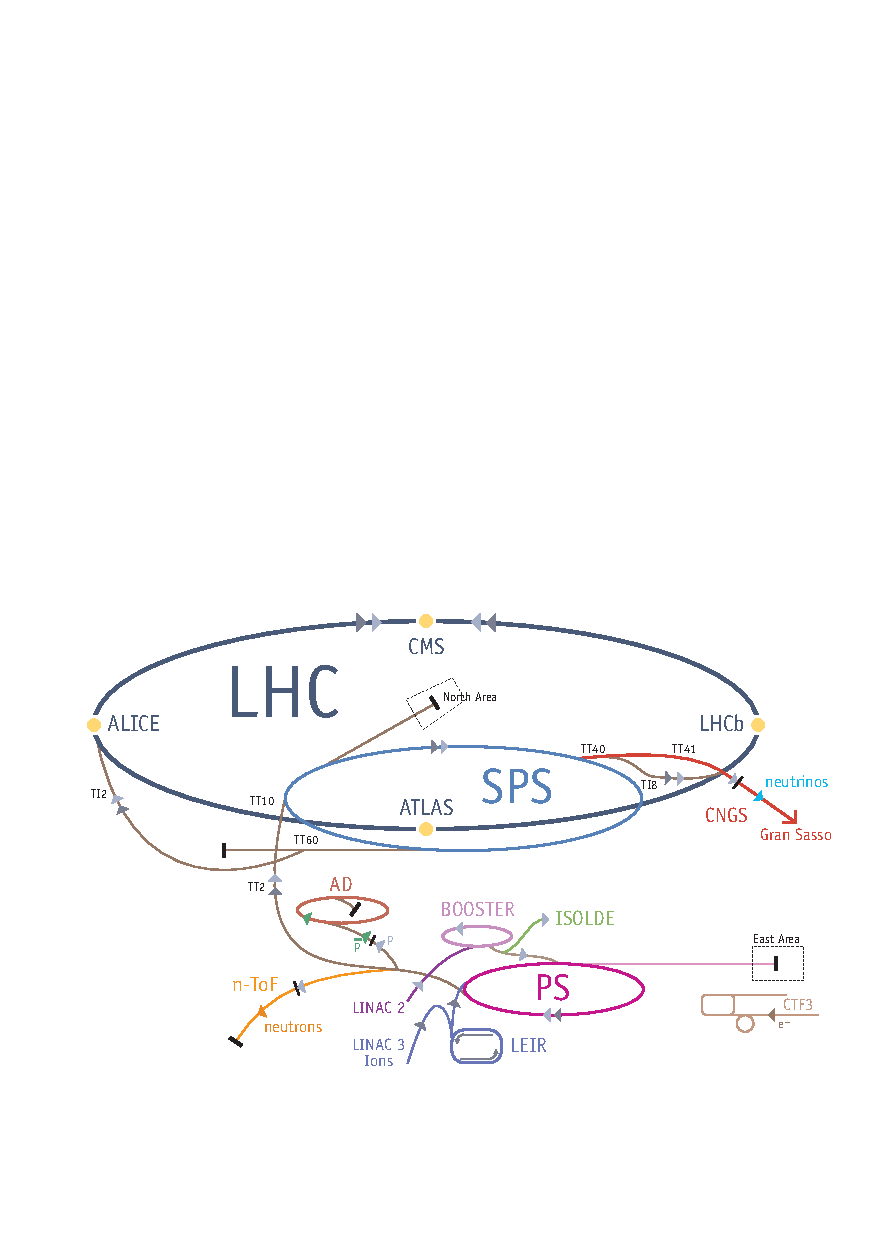
\includegraphics[width=\columnwidth]{LHC}
  \caption{CERN accelerator complex}
  \label{fig:LHC}
\end{figure}
\newpage
A schematic view of the LHC accelerator chain is shown in Figure~\ref{fig:LHC}. Initially, the protons are obtained by
stripping orbiting electrons from hydrogen atoms. Then they are injected into the linear accelerator LINAC2 to reach the
energy of \SI{50}{\MeV} and enter the Proton Synchrotron Booster (PSB). The booster accelerates them to \SI{1.4}{\GeV}
and passes the beam to the Proton Synchrotron (PS) where the energy rises to \SI{25}{\GeV}. In the next step, protons
enter the Super Proton Synchrotron (SPS) where they are accelerated to \SI{450}{\GeV}. Finally, the beam is transferred
to the LHC in both clockwise and anti-clockwise directions where it takes about 20 minutes to reach the design
\SI{7}{\TeV} energy (per beam).

The LHC has four interaction points, providing collisions to four major experiments. Two of them, CMS and ATLAS, are
multi-purpose high-luminosity experiments with a peak luminosity of $\calL = $ \SI{d34}{\cm^{-2} s^{-1}}. The other two
experiments operate at low luminosities and have more specific physics goals: LHCb studies b-meson decays, and Alice is
a dedicated heavy ion experiment.

The instantaneous luminosity of a collider can be calculated as
\begin{equation}
	\calL = \frac{n_1 n_2 n_b f}{4 \pi \sigma_x \sigma_y},
\end{equation}
where $n_1$ and $n_2$ are the numbers of particles in each of the colliding bunches, $n_b$ is the number of bunches per
beam, $f$ is the revolution frequency, $\sigma_x$ and $\sigma_y$ are the horizontal and vertical beam sizes, assuming
the two beams have the same size. These and other performance-related parameters of the LHC for different running
conditions are shown in Table~\ref{tab:LHC_parameters}.

The number of events generated in the collisions per second is given by
\begin{equation}
	N_{events} = \calL \times \sigma,
\end{equation}
where $\sigma$ is the cross section of the process under study. Cross sections and production rates for several
different processes as a function of the centre of mass energy are shown in Figure~\ref{fig:production_cross_sections}.

\begin{table}[!htbp]
\centering
\caption[LHC beam parameters]{LHC beam parameters \autocite{LHC_design_report, CERN_courier_LHC_run}. Transverse beam
size and peak luminosity quoted at interaction points 1 and 5 (ATLAS and CMS detectors).}
\label{tab:LHC_parameters}
\begin{tabular}{|lrrr|}
  \toprule
                                              & 2011 run & 2012 run & Design value \\
  \midrule
  Beam energy (\si{\TeV})                     & \num{3.5}         & \num{4}           & \num{7}       \\
  Maximum number of bunches                   & \num{1380}        & \num{1380}        & \num{2808}    \\
  Number of particles per bunch               & \num{1.45e11}     & \num{1.7e11}      & \num{1.15e11} \\
  Bunch spacing (\si{\nano\s})                & \num{75/50}       & \num{50}          & \num{25}      \\
  Revolution frequency (\si{\kilo\hertz})     & \num{11.245}      & \num{11.245}      & \num{11.245}  \\
  Transverse beam size (\si{{\micro\metre}})  & \num{25.9}        & \num{18.8}        & \num{16.7}    \\
  Peak luminosity (\si{\cm^{-2}~\s^{-1}})     & \num{3.7e33}      & \num{7.7e33}      & \num{e34}     \\
  \bottomrule
\end{tabular}
\end{table}

\newpage
\begin{figure}[!htbp]
  \centering
  \leavevmode
  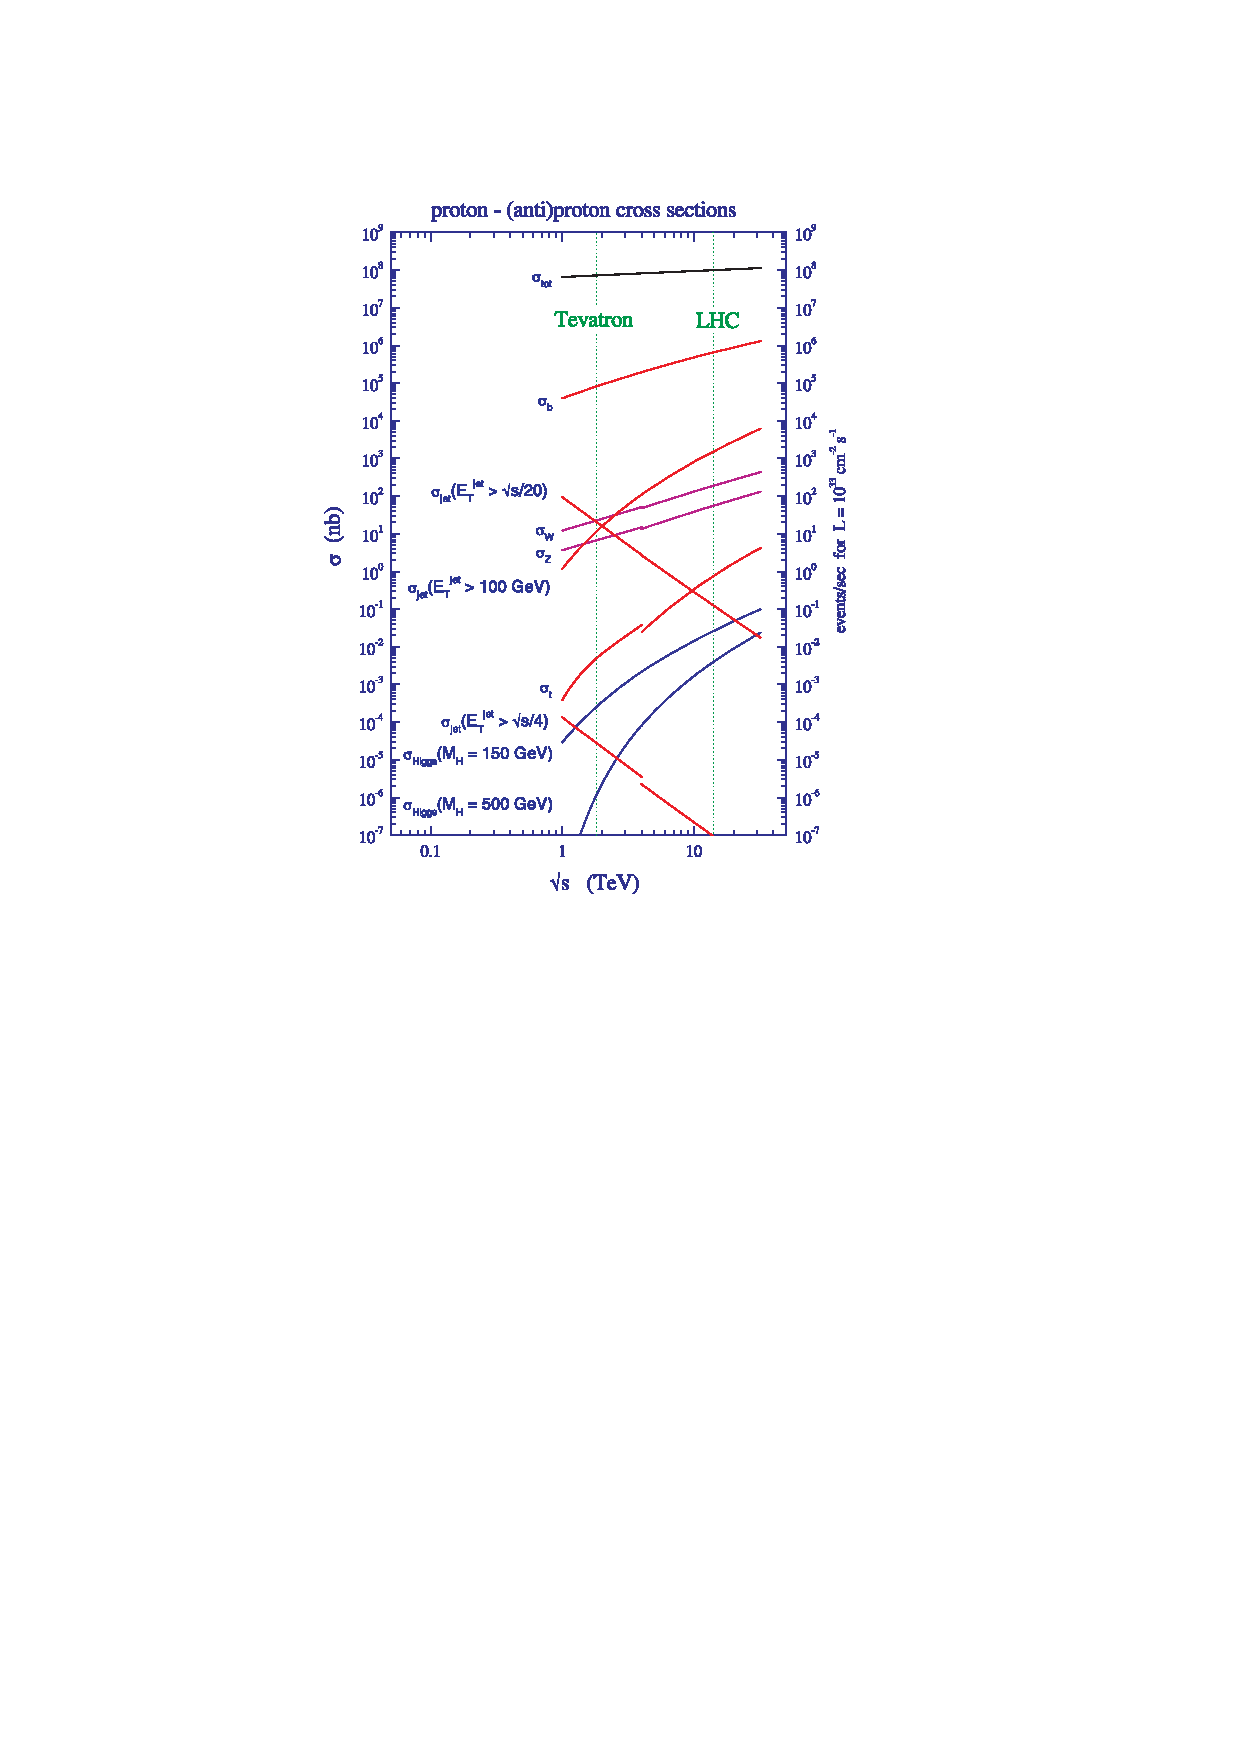
\includegraphics[width=0.7\columnwidth]{production_cross_sections}
  \caption[Production cross sections for different processes as a function of the centre of mass energy]{Production
  cross sections for different processes as a function of the centre of mass energy $\sqrt{s}$. The discontinuity is due
  to extrapolation between proton-antiproton Tevatron and proton-proton LHC. The \ttbar production cross section is
  denoted by $\sigma_\textrm{t}$ \autocite{primer_LHC}.}
  \label{fig:production_cross_sections}
\end{figure}

The LHC started operating on 10 September 2008 with the first beams fully circulating in both rings. However, only nine
days later a magnet quench occurred in two sectors of the tunnel, which was caused by an electrical fault due to a bad
connection between two magnets. A consequent liquid helium explosion damaged a total of 53 superconducting magnets. Over
a year was spent on repairs and tests, and the first collisions were recorded on 23 November 2009 at a centre of mass
energy of \SI{0.9}{\TeV}. The following few months showed the continuous ramp up of the beam energies up to
\SI{3.5}{\TeV} per beam which was achieved on 30 March 2010 when the LHC physics programme started.

Throughout the rest of 2010, the two general-purpose LHC experiments (CMS and ATLAS) recorded approximately
\SI{40}{\invpb} of data, which resulted in the first measurements of various physics processes at the LHC. The following
year became the main \SI{7}{\TeV} data-taking period, with about \SI{5}{\invfb} of data recorded by ATLAS and CMS. On 5
April 2012 the centre of mass energy was increased to 8 TeV, and July of 2012 marked the first major discovery of a new
boson which was later shown to be consistent with the Standard Model Higgs boson, according to approximately
\SI{21.8}{\invfb} of data recorded until early 2013. A long shut-down is planned for the following two years with
various upgrades scheduled. The next physics run is expected in 2015 with the beam energy increased up to 6 or
\SI{7}{\TeV}.

\section{The CMS Detector}
\label{s:CMS}

The Compact Muon Solenoid \autocite{CMS} is a general-purpose detector designed to carry out precise measurements of the
Standard Model and searches for physics beyond it. The primary design requirement was the ability to discover the nature
of electroweak symmetry breaking, and the first observation of a Higgs boson was obtained in the Summer of 2012
\autocite{CMS_higgs_observation}.

The detector is installed at one of the LHC interaction points (Point 5) at about \SI{100}{\metre} underground near the
French village of Cessy, between the Jura mountains and Lake Geneva. The overall dimensions of the CMS detector are a
length of \SI{21.6}{\metre}, a diameter of \SI{14.6}{\metre} and a total weight of \SI{12500}{\tonne}.

\begin{figure}[htbp]
  \centering
  \leavevmode
  \includegraphics[width=\columnwidth]{CMS}
  \caption{Sectional view of the CMS detector}
  \label{fig:CMS}
\end{figure}

The sectional view of CMS is shown in Figure~\ref{fig:CMS}. In the centre of the detector, tracking and calorimetry
systems are surrounded by the superconducting solenoid. On the outermost part of it the magnetic flux is returned
through the iron yoke in which the muon system is also integrated. All the sub-systems are discussed in the following
sections in more detail.

The cylindrical shape of the CMS detector dictates using a cylindrical coordinate system, with the origin centred at the
interaction point, the $x$-axis pointing towards the centre of the LHC ring, the $y$-axis pointing upwards and the
$z$-axis pointing along the beamline in the anti-clockwise direction. The azimuthal angle $\phi$ is measured from the
$x$-axis in the transverse ($x-y$) plane and the polar angle $\theta$ is measured from the $z$-axis. The radial distance
to the beamline is denoted by $r$. Pseudorapidity is defined as:
\begin{equation}
  \eta = - \ln{\tan{\frac{\theta}{2}}}.
\end{equation}
This implies that the particles moving in the transverse plane (perpendicular to the beamline) have a pseudorapidity of
0, whereas the beam direction has an infinite pseudorapidity. Considering the cylindrical shape of the detector, it has
barrel and endcap regions, with the transition occurring at $\eta \sim 1.4$. The momentum and energy transverse to the
beamline are denoted by $p_T$ and $E_T$ respectively; the imbalance of the energy measured in the transverse plane,
called missing transverse energy, is denoted by \MET.

The distance between any two objects (say, $i$ and $j$) in the detector is often described in terms of $\Delta R$
quantity, defined as follows:
\begin{equation}
  \Delta R = \sqrt{(\eta_i-\eta_j)^2 + (\phi_i-\phi_j)^2}.
\end{equation}
The same quantity will be used to define cones in jet clustering algorithms, described in
Section~\ref{ss:jet_reconstruction}.

\subsection{Inner Tracking System}
\label{ss:tracker}
The tracking system lies in the heart of the CMS detector and is the closest to the interaction point where the particle
flux has the highest value. This imposes demanding requirements on the configuration of the system. At design luminosity
of $\calL = $ \SI{d34}{\cm^{-2}~\s^{-1}} with the bunch spacing of \SI{25}{\ns}, an average of \num{1000} particles from
about \num{25} proton-proton interactions (pile-up vertices) is expected to traverse the tracker for each bunch
crossing. However, up until the long shutdown a bunch spacing of \SI{50}{\ns} was used, which meant a higher number of
protons in each bunch leading to approximately twice the number of pile-up vertices. Therefore, in order for the
particle tracks to be identified reliably and separately for each bunch crossing, the tracker requires very fine
granularity and fast response parameters. Another complication caused by the intense particle flux is the severe
radiation damage, so the tracker has to be highly resilient in operating in the harsh environment for a reasonable
lifetime.

To meet these requirements on granularity, response time and radiation resilience, the tracker design was chosen to be
based on silicon detector technology. Although capable of meeting such conditions, this technology has a disadvantage of
a high power density of on-detector electronics. This implies the necessity of an efficient cooling system. Moreover, a
large amount of dense material interacting with the particles leads to higher multiple scattering, bremsstrahlung,
photon conversions and nuclear interactions. Therefore, there are complications in the reconstruction of the tracks,
meaning some loss of efficiency and precision. This will be discussed in detail later on in the object reconstruction
section.

\begin{figure}[htbp]
  \centering
  \leavevmode
  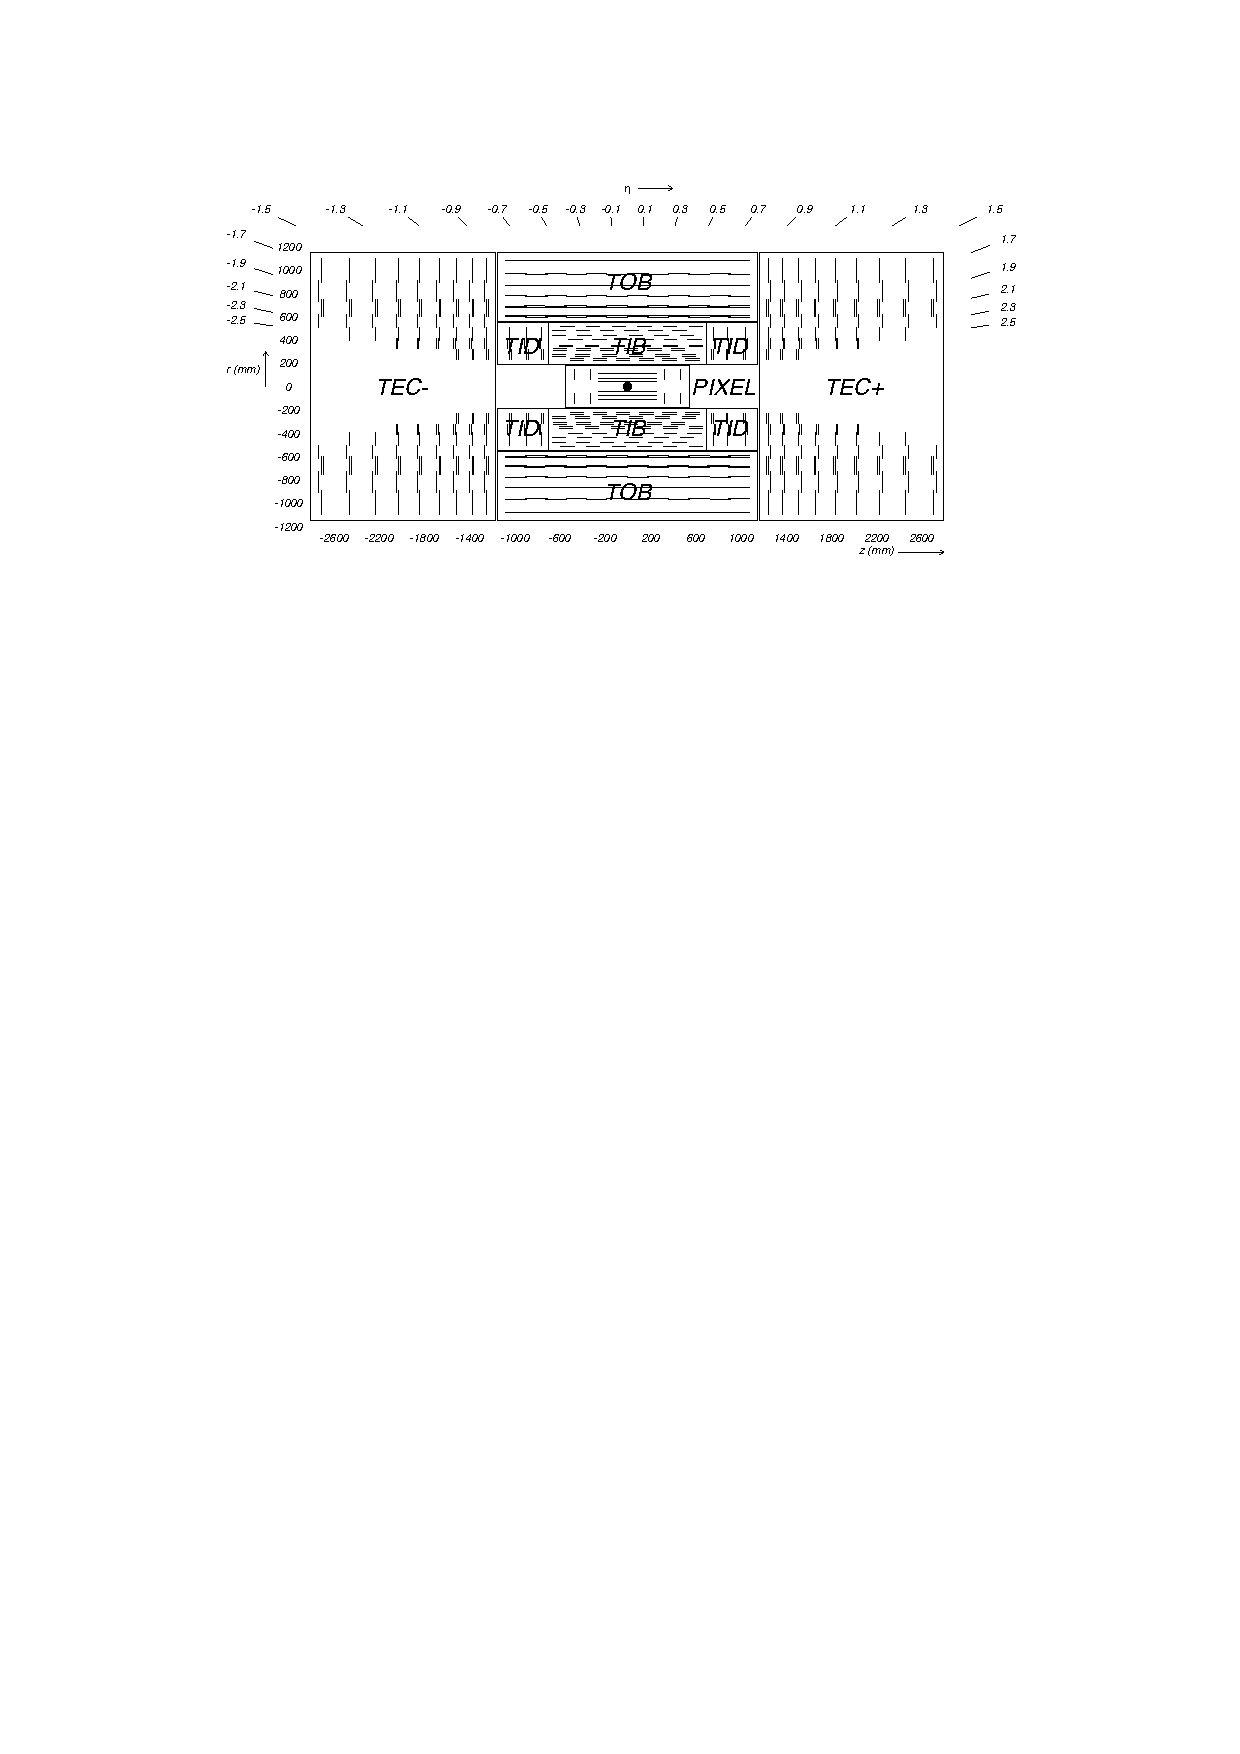
\includegraphics[width=\columnwidth]{tracker}
  \caption[Cross section of the CMS tracker system]{Cross section of the CMS tracker system \autocite{CMS}}
  \label{fig:tracker}
  \vspace*{1ex}
\end{figure}

Figure~\ref{fig:tracker} shows the overall layout of the tracking system. It consists of the inner pixel detector,
located in the vicinity of the interaction point, and silicon strip tracker detectors: inner barrel and disks (TIB and
TID), outer barrel (TOB) and endcaps (TEC). The geometrical acceptance of the tracker system goes up to \abs\eta
\num{<2.5}. The outer radius of the CMS tracker reaches approximately \SI{110}{\cm}, and its total length is about
\SI{540}{\cm}.

The pixel detector consists of three layers of pixel sensors at radii of \SIlist{4.4;7.3;10.2}{\cm} from the beamline in
the barrel region. In addition there are two endcap disks on each side at \abs z $=$ \SIlist{34.5;46.5}{\cm}. The pixel
size equals \num{100x150} \si{\micron\squared} in $r \phi \times z$ coordinates. The pixel detector has 66 million
pixels and the total area of about \SI{1}{\m\squared}.

The silicon strip tracker consists of several layers of silicon microstrip detectors. It covers the region between
\SIrange{20}{110}{\cm} in radius and extends up to \SI{+-280}{\cm} in the z direction. The Tracker Inner Barrel (TIB) is
made out of 4 layers and the Tracker Outer Barrel (TOB) has 6 layers in it. The tracker endcaps (TEC) comprise 9 disks,
and there are also the tracker inner disks (TID) that consist of 3 disks filling the gap between TIB and TEC as shown in
Figure~\ref{fig:tracker}. There are \num{9.3} million silicon strips covering the area of about \SI{200}{\m\squared}.
The silicon sensors' thickness varies between \num{320} and \SI{500}{\micron} and the strip pitch varies from
\SI{80}{\micron} in the TIB to \SI{180}{\micron} in TOB and TEC.

\begin{figure}[!htbp]
  \centering
  \leavevmode
  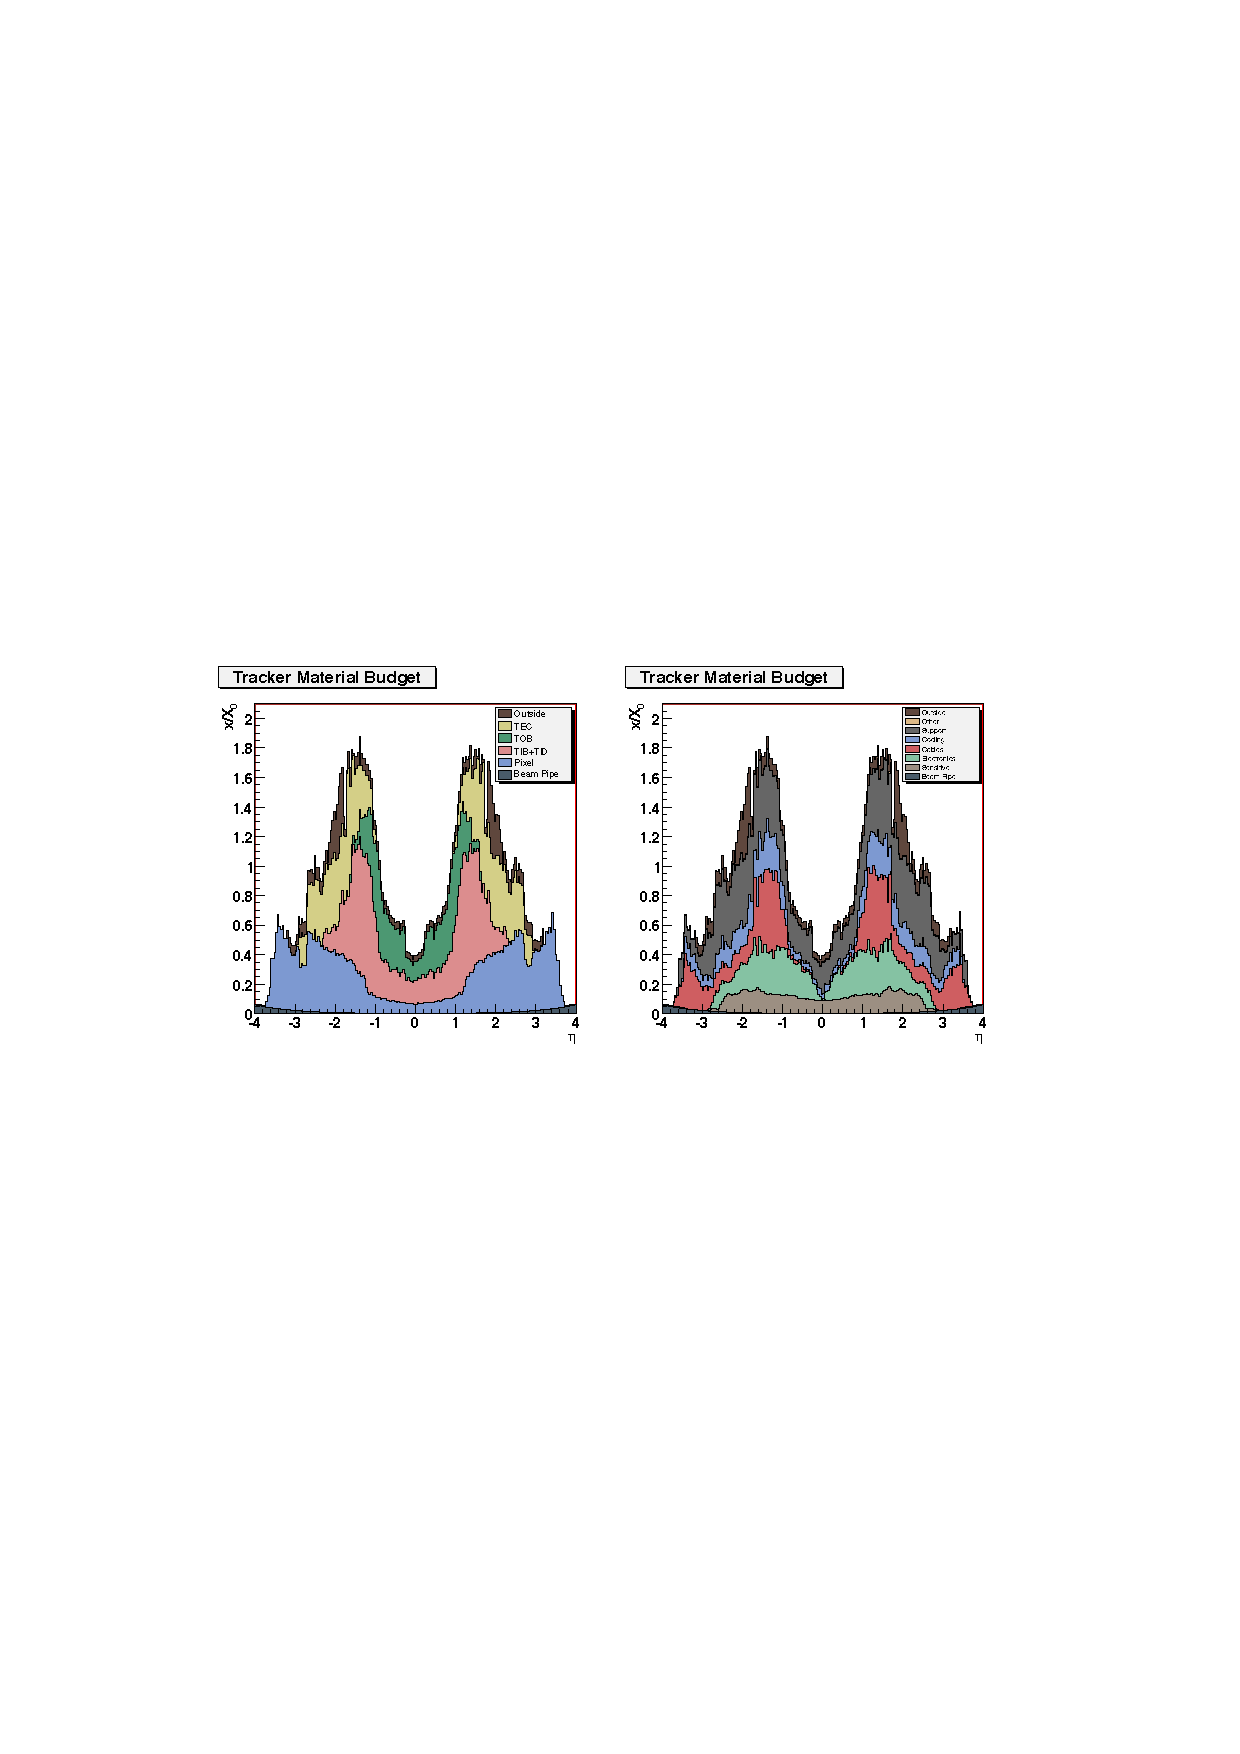
\includegraphics[width=0.6\columnwidth]{tracker_material_budget}
  \caption[Material budget as a function of pseudorapidity $\eta$ for the different sub-detectors of the
  tracker]{Material budget as a function of pseudorapidity $\eta$ for the different sub-detectors of the tracker in
  units of radiation length \autocite{CMS_tracker_twiki}}
  \label{fig:tracker_material_budget}
\end{figure}

The silicon detectors of the tracker, the readout electronics and support structure form a considerable amount of
material for the particles traversing from the interaction point. Figure~\ref{fig:tracker_material_budget}
\autocite{CMS} shows the material budget of the CMS tracker in units of radiation lengths\footnote{A material's
radiation length is the mean distance over which a high-energy electron loses all but $1/e$ of its energy by
bremsstrahlung; this is equal to \num{7/9} of the mean free path for pair production by a high-energy photon.} ($X_0$).
It grows from about \num{0.4} $X_0$ to \num{1.8} $X_0$ in the barrel region, and then decreases to about \num{1} $X_0$
in the endcaps. This causes a substantial conversion rate for photons and electrons in the tracker material; it also
will be discussed in more detail in the electron reconstruction section.

%\textit{[perhaps need to add the $p_T$ resolution plots]}

\subsection{Electromagnetic Calorimeter}
The next detector subsystem which is surrounding the tracker is the electromagnetic calorimeter, or ECAL. It is of a
primary importance for the analyses described in this thesis, as it provides information for the electron and positron
reconstruction. Combination of this information with that from the tracking system must ensure a precise measurement of
electron position and momentum, and also sufficient background removal. It has to effectively distinguish the energy
deposit shape of an electromagnetic particle from the one of a hadronic particle, which requires good segmentation and
high resolution.

ECAL is a hermetic, high-granularity, high-resolution scintillating crystal calorimeter consisting of \num{61200} lead
tungstate ($\textrm{PbWO}_4$) crystals located in the central barrel region (\abs\eta $<1.479$), and \num{7324} crystals
in each of the two endcaps (\num{1.479} $<$\abs\eta\num{<3.0}). All crystals are followed by photodetectors reading and
amplifying their scintillation: avalanche photodiodes (APD) are used in the barrel, and vacuum phototriodes (VPTs) are
used in the endcaps. These different choices were caused by the configuration of the magnetic field and the expected
level of radiation.

\begin{figure}[!htbp]
  \centering
  \leavevmode
  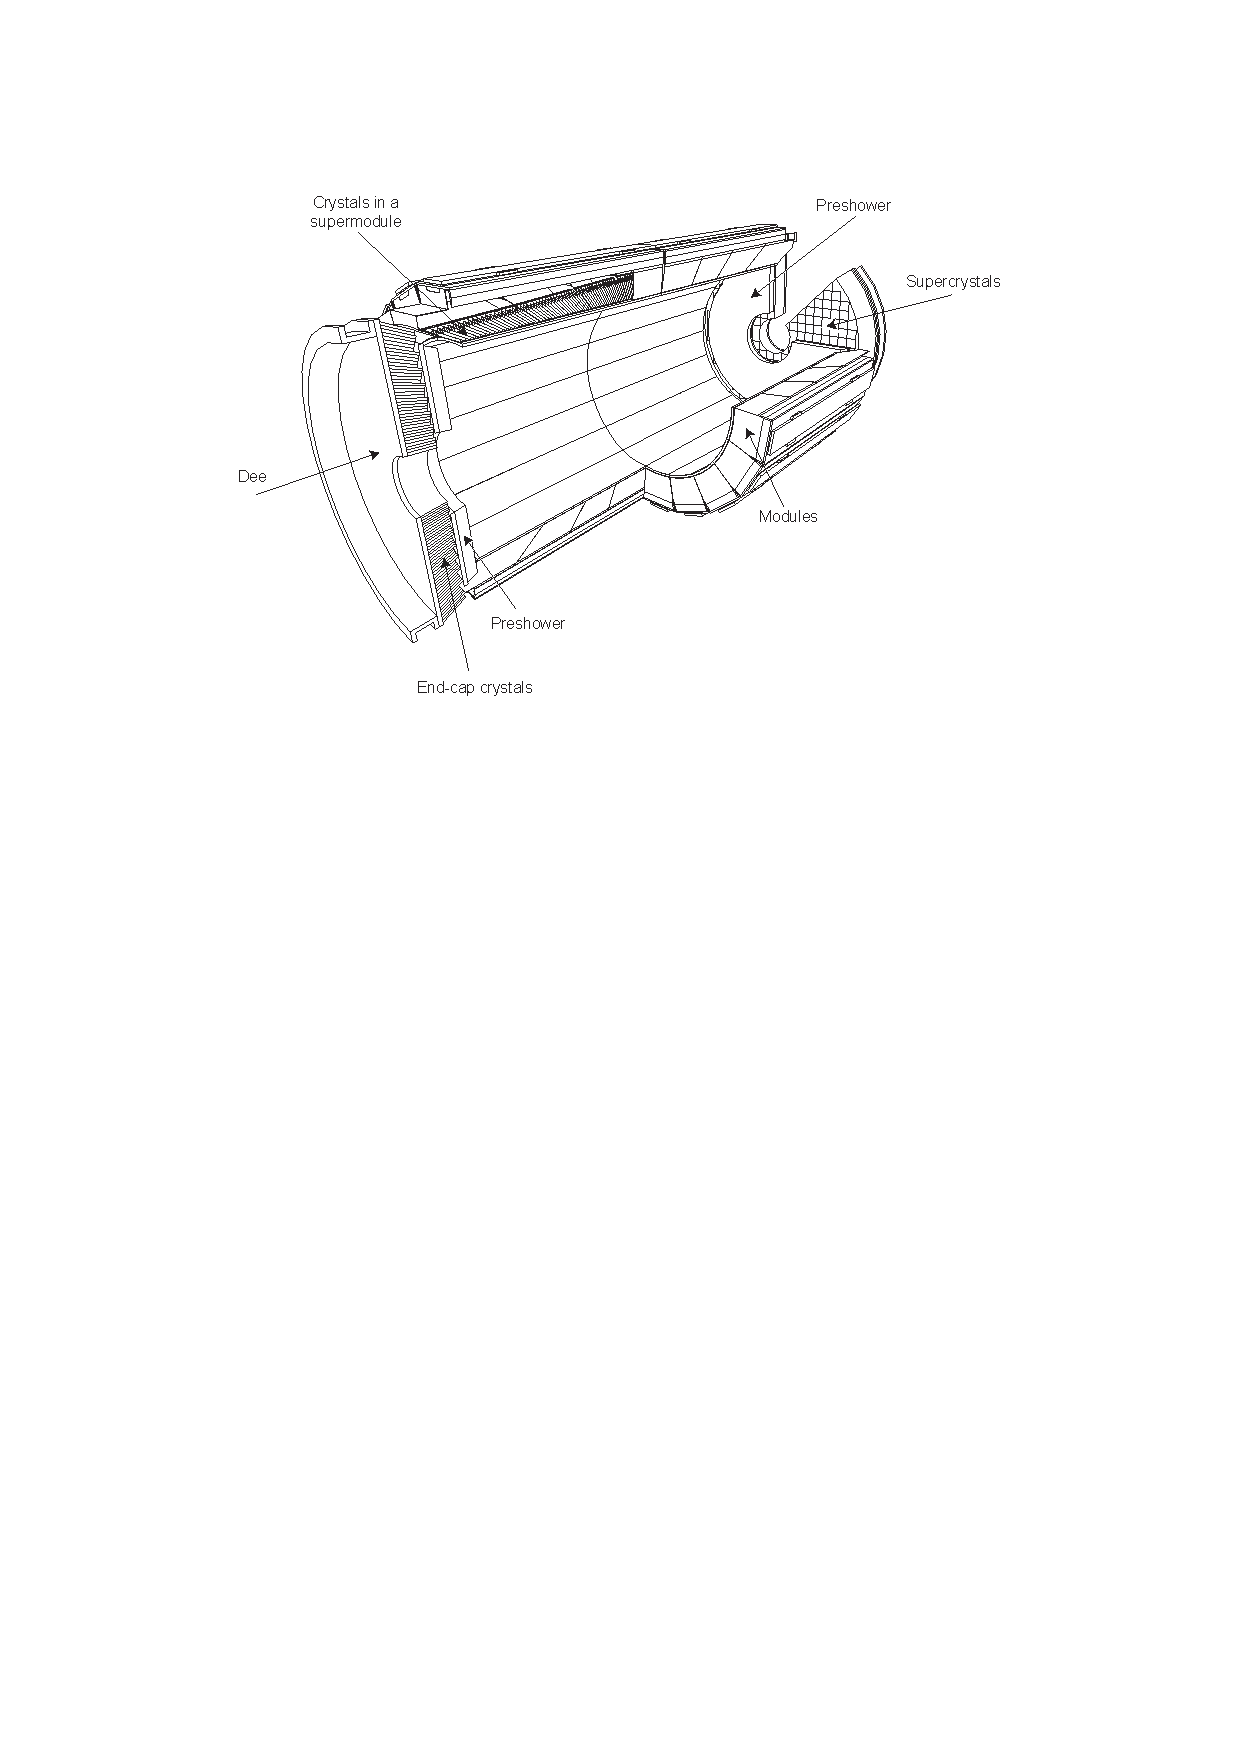
\includegraphics[width=\columnwidth]{ECAL}
  \caption[Layout of the CMS electromagnetic calorimeter]{Layout of the CMS electromagnetic calorimeter \autocite{CMS}}
  \label{fig:ECAL}
\end{figure}

The layout of the ECAL sub-detector is shown in Figure~\ref{fig:ECAL}. An additional preshower detector is used in the
endcap region to lower the required detector depth. Its principal aim is to identify neutral pions in the endcaps, but
it also helps to distinguish neutral pions and electrons from minimum ionising particles and improves the position
determination of electrons and photons with high granularity.

\begin{table}[htbp]
\centering
\caption[ECAL crystal characteristics]{ECAL crystal characteristics \autocite{CMS_TDR1}}
\label{tab:ECAL_crystals}
\begin{tabular}{|lrr|}
  \toprule
   & Barrel & Endcaps \\
  \midrule
  Number of crystals & \num{61200} & \num{14648} \\
  Crystal cross section in ($\eta$, $\phi$) & \num{0.0174 x 0.0174} & varies \\
  Crystal cross section at the front & \num{22x22} \si{\mm\squared} & \num{28.62x28.62} \si{\mm\squared} \\
  Crystal cross section at the rear & \num{26x26} \si{\mm\squared} & \num{30x30} \si{\mm\squared} \\
  Crystal length & \SI{230}{\mm} (\num{25.8}$X_0$) & \SI{220}{\mm} (\num{24.7}$X_0$) \\
  \bottomrule
\end{tabular}
\end{table}

The main geometrical characteristics of the ECAL crystals are shown in Table~\ref{tab:ECAL_crystals}. The choice of lead
tungstate was driven by the constraints of the CMS design. It is a very dense material (\SI{8.28}{g\per\cm\cubed}) with
a short radiation length of $X_0 = \SI{0.89}{\cm}$, which allows the calorimeter to fit inside the compact magnet. Lead
tungstate also has a small Moli\`ere radius\footnote{The Moli\`ere radius $R_\mu$ is a characteristic constant of a
material giving the scale of the transverse dimension of the fully contained electromagnetic showers initiated by an
incident high energy electron or photon. It is defined as the radius of a cylinder containing an average of
\SI{90}{\percent} of the shower's energy deposition.} of \SI{2.2}{\cm}, which allows a calorimeter with fine
granularity. Finally, the crystals emit \SI{80}{\percent} of their scintillation light in just \SI{25}{\ns}, however the
light yield is relatively low. At \SI{18}{\degreeCelsius}, about \num{4.5} photoelectrons per MeV are collected. The
dependence of the light yield on temperature requires a cooling system capable of keeping the crystal temperature stable
within \SI{+-0.05}{\degreeCelsius} to preserve energy resolution \autocite{CMS_TDR1}.

The energy-dependent resolution of the calorimeter can be parameterised as follows \autocite{CMS}:
\begin{equation}
  \left(\frac{\sigma}{E}\right)^2 = \left(\frac{S}{\sqrt E}\right)^2 + \left(\frac{N}{E}\right)^2 + C^2.
\end{equation}
where $S$ is the stochastic term, $N$ is the noise term, and $C$ is the constant term. Figure~\ref{fig:ECAL_resolution}
shows the energy resolution in bins of pseudorapidity, measured using $\Z \rightarrow ee$ decays from MC simulation and
2012 data.

\begin{figure}[htbp]
  \centering
  \leavevmode
  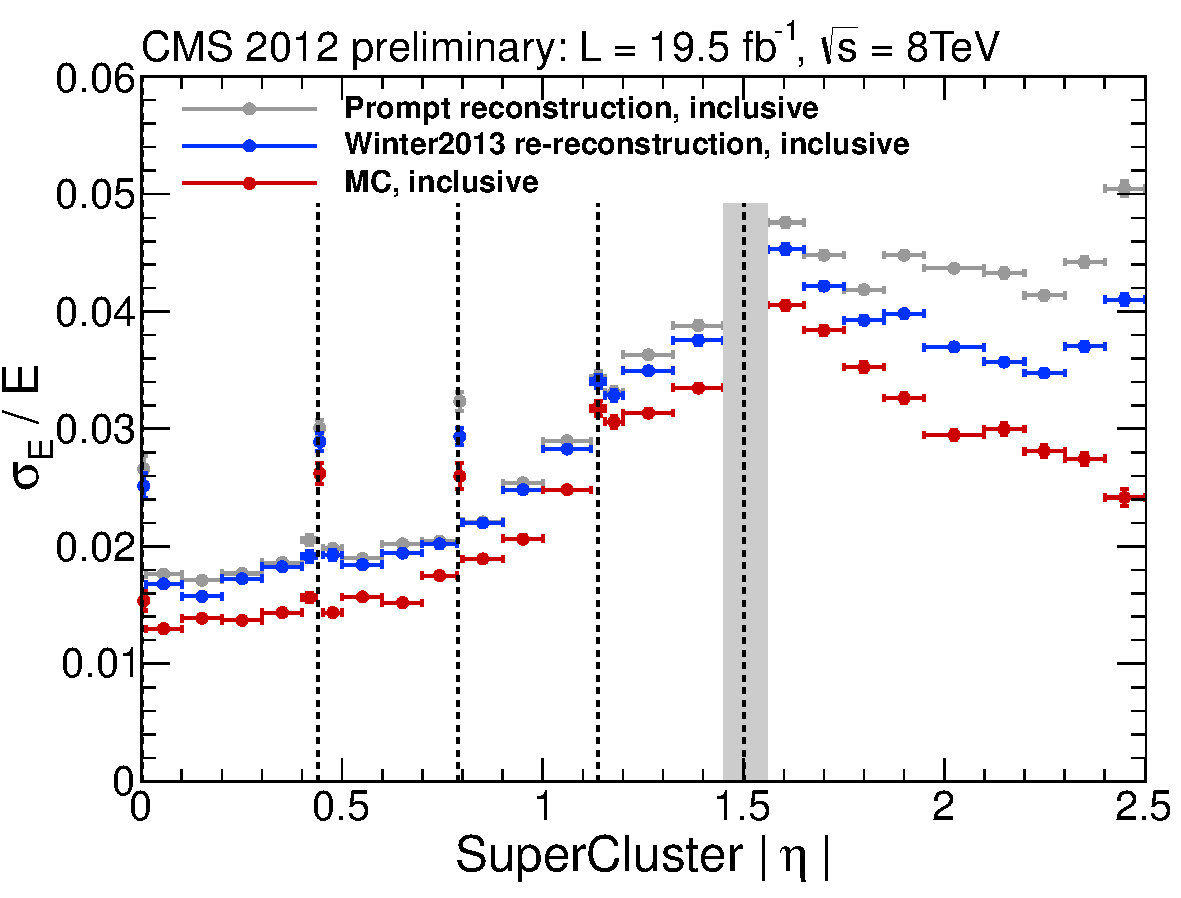
\includegraphics[width=0.7\columnwidth]{ECAL_resolution}
  \caption[Relative ECAL energy resolution in bins of pseudorapidity $\eta$]{Relative electron (ECAL) energy resolution
unfolded in bins of pseudorapidity $\eta$. Electrons from $\Z \rightarrow ee$ decays are used. The resolution
$\sigma_\mathrm{E}/\mathrm{E}$ is plotted separately for data and simulated events \autocite{CMS_ECAL_twiki}.}
  \label{fig:ECAL_resolution}
\end{figure}

\subsection{Hadron Calorimeter}

The hadron calorimeter (HCAL) is the next sub-detector located mostly inside the solenoid and completing the CMS
calorimetry system. It is essential for the measurement of hadron jets and missing transverse energy.

\begin{figure}[htbp]
  \centering
  \leavevmode
  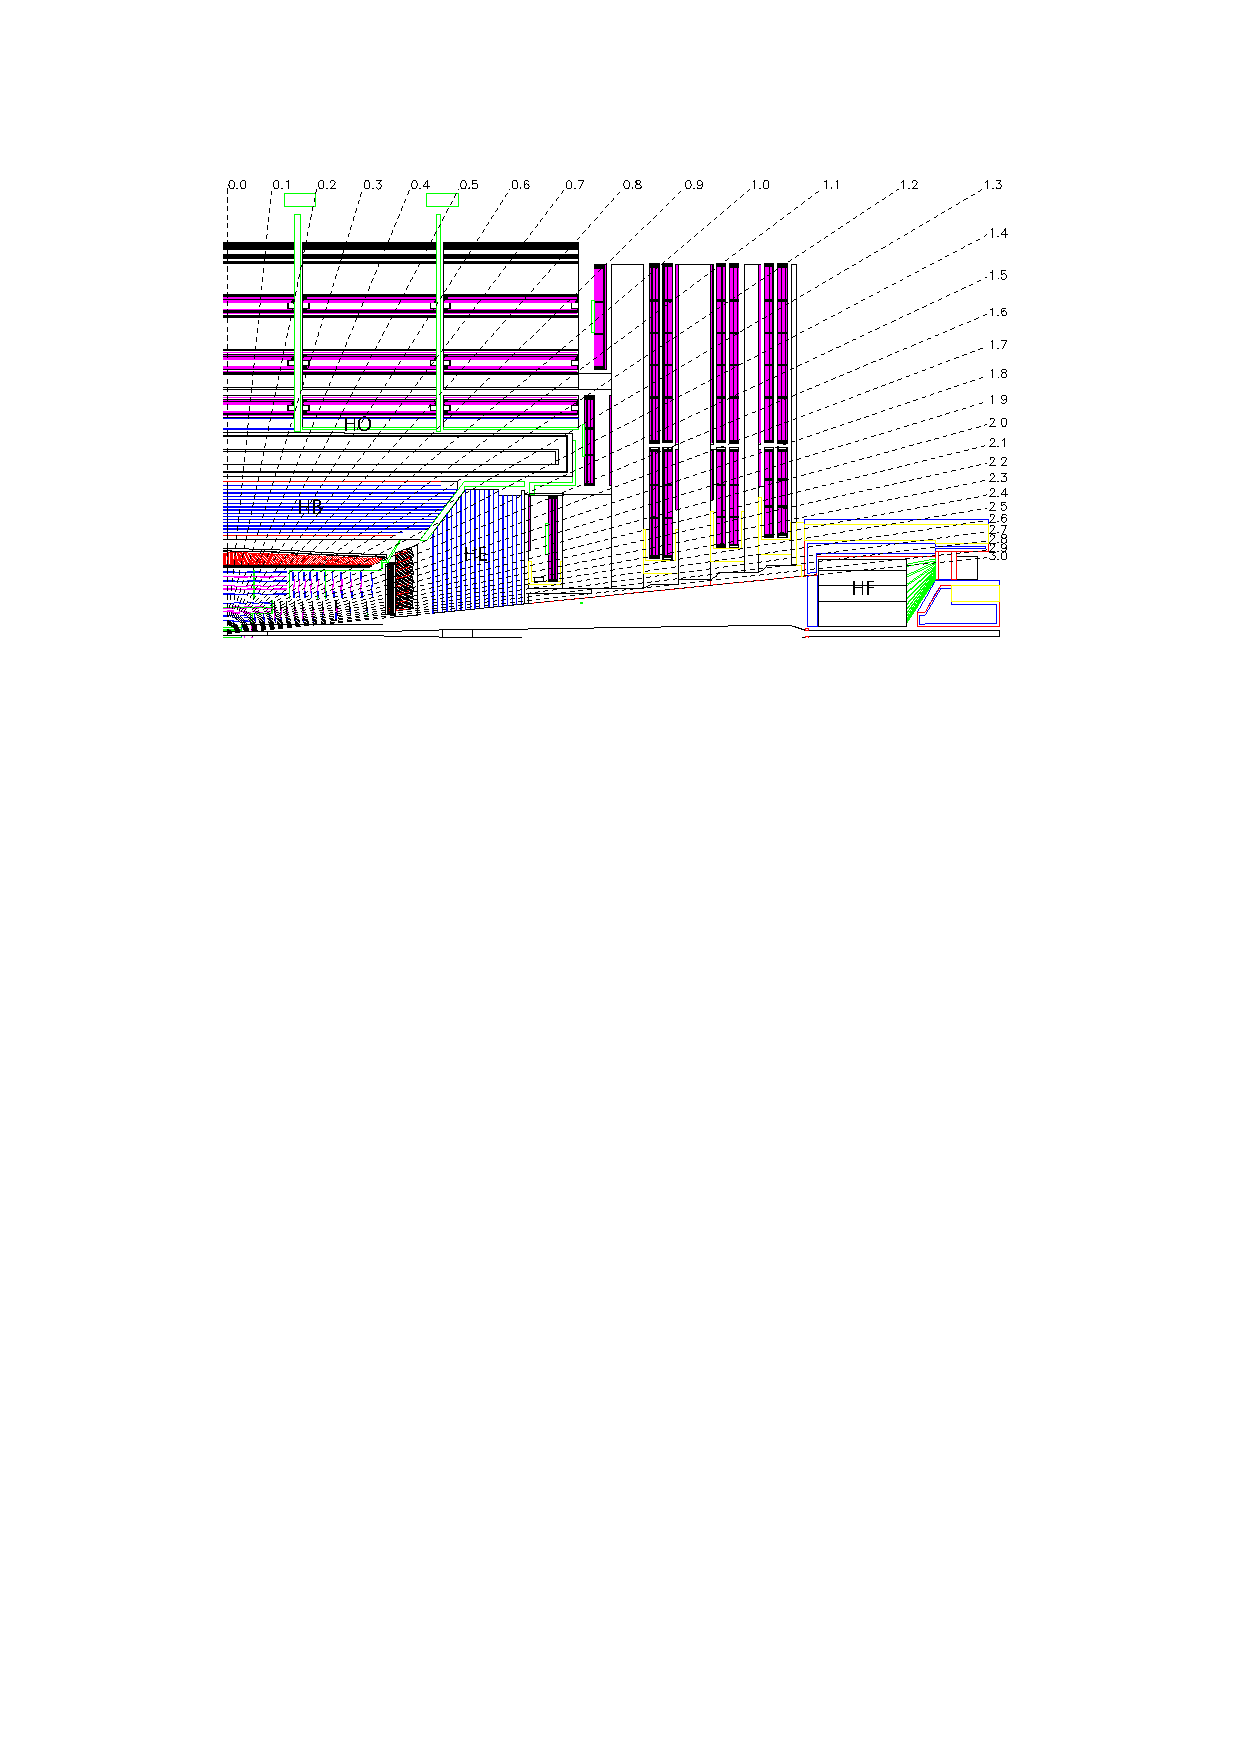
\includegraphics[width=\columnwidth]{HCAL}
  \caption[Longitudinal view of the CMS detector]{Longitudinal view of the CMS detector showing the locations of the
  hadron barrel (HB), endcap (HE), outer (HO) and forward (HF) calorimeters \autocite{CMS}.}
  \label{fig:HCAL}
\end{figure}

As shown in Figure~\ref{fig:HCAL}, HCAL consists of four subsystems: the hadron barrel calorimeter (HB), the hadron
endcap calorimeter (HE), the hadron outer calorimeter (HO) and the hadron forward calorimeter (HF). The barrel and
endcap parts (HB, HE) cover the pseudorapidity range up to \abs\eta \num{<3.0}, and the forward part (HF) extends it to
a total coverage of \abs\eta \num{<5.0}. HCAL surrounds ECAL from its outer limit of \SI{1.77}{\metre} from the
beamline, to the inner limit of the magnet coil at \SI{2.95}{\metre} from the beamline. However, due to space
limitations the barrel calorimeters do not contain complete hadronic showers, therefore an outer calorimeter (HO) was
designed to measure the energy leakage. It is placed in the muon system just outside of the solenoid in the barrel
region.

HCAL is a sampling calorimeter consisting of alternating layers of brass and stainless steel absorbers, and plastic
scintillators as active elements. The choice of the absorber material was caused by its short hadronic interaction
length and its property of being non-magnetic, which is crucial in the strong magnetic field of the CMS magnet. The
scintillation light is guided by embedded wavelength-shifting (WLS) fibres. The light from the WLS is then transmitted
via a network of clear fibres, arranged in read-out towers, to hybrid photodiodes (HPDs) \autocite{CMS}.

Both HB and HE scintillators have a granularity of $\Delta \eta \times \Delta \phi =$ \num{0.087x0.087} for \abs\eta
\num{<1.6}, and $\Delta \eta \times \Delta \phi =$ \num{0.17x0.17} for \abs\eta \num{>=1.6}. The tower segmentation of
the forward calorimeter (HF) varies from $\Delta \eta \times \Delta \phi =$ \num{0.175x0.175} at \abs\eta \num{=3.0} to
$\Delta \eta \times \Delta \phi =$ \num{0.3x0.35} at at \abs\eta \num{=5.0}. The HF is placed at about \SI{11}{\metre}
from the interaction point, and is essential to reconstruct very forward hadron jets. Together with HO, it provides the
hermeticity of the calorimetry system, making it possible to measure the transverse missing energy to a reasonable
precision.

%\textit{[Can't find recent resolution plots]}

\subsection{Superconducting Magnet}
The superconducting solenoid is a central feature of the CMS apparatus, essentially giving it its name. The magnet
has a length of \SI{12.5}{\metre}, diameter of \SI{6.3}{\metre} and mass of \SI{220}{\tonne}. Although it was initially
designed to sustain a uniform magnetic field of \SI{4}{\tesla} within the \SI{5.9}{\metre} diameter free bore, operation
at \SI{3.8}{\tesla} was chosen in order to increase the lifetime. The magnetic field is returned by a massive iron yoke.
The main parameters of the CMS magnet are shown in Table~\ref{tab:solenoid_parameters}.

\begin{table}[htbp]
\caption[Parameters of the CMS superconducting solenoid]{Parameters of the CMS superconducting solenoid \autocite{CMS_TDR1, CMS_Solenoid}}
\label{tab:solenoid_parameters}
\centering
\begin{tabular}{@{}lr@{}}
  \toprule
  Parameter & Value \\    
  \midrule
  Field & \SI{3.8}{\tesla} \\
  Inner bore & \SI{5.9}{\metre} \\
  Length & \SI{12.5}{\metre} \\
  Number of turns & \num{2168} \\
  Current & \SI{18160}{\kilo\ampere} \\
  Stored energy & \SI{2.3}{\giga\joule} \\
  \bottomrule
\end{tabular}
\end{table}


The large bending power of the solenoid is required to bend the tracks of high energy charged particles to an extent
where good momentum resolution is achieved. The design requirement for the strength of the magnetic field was the
ability to unambiguously determine the sign of the electric charge for muons with a momentum of \SI{\approx 1}{\TeV/c}
\autocite{CMS_TDR1}.

The solenoid coil is constructed from four layers of superconducting high-purity niobium-titanium cable co-extruded with
pure aluminium, which acts as a thermal stabiliser. The cold mass is cooled down to \SI{4.5}{K} by liquid helium. If a
fast discharge happens (e.g.\ caused by a magnet quench), about 3 days are necessary to re-cool the coil.

\subsection{Muon System}
The last sub-detector placed on the outermost part of CMS is the muon system. Since the muons are the most penetrating
particles detectable by CMS, they have the cleanest signature and play an important role in many physics analyses. Due
to their ability to travel through the many layers of the calorimeters, muons are relatively easy to identify and
separate from the background.

\begin{figure}[htbp]
  \centering
  \leavevmode
  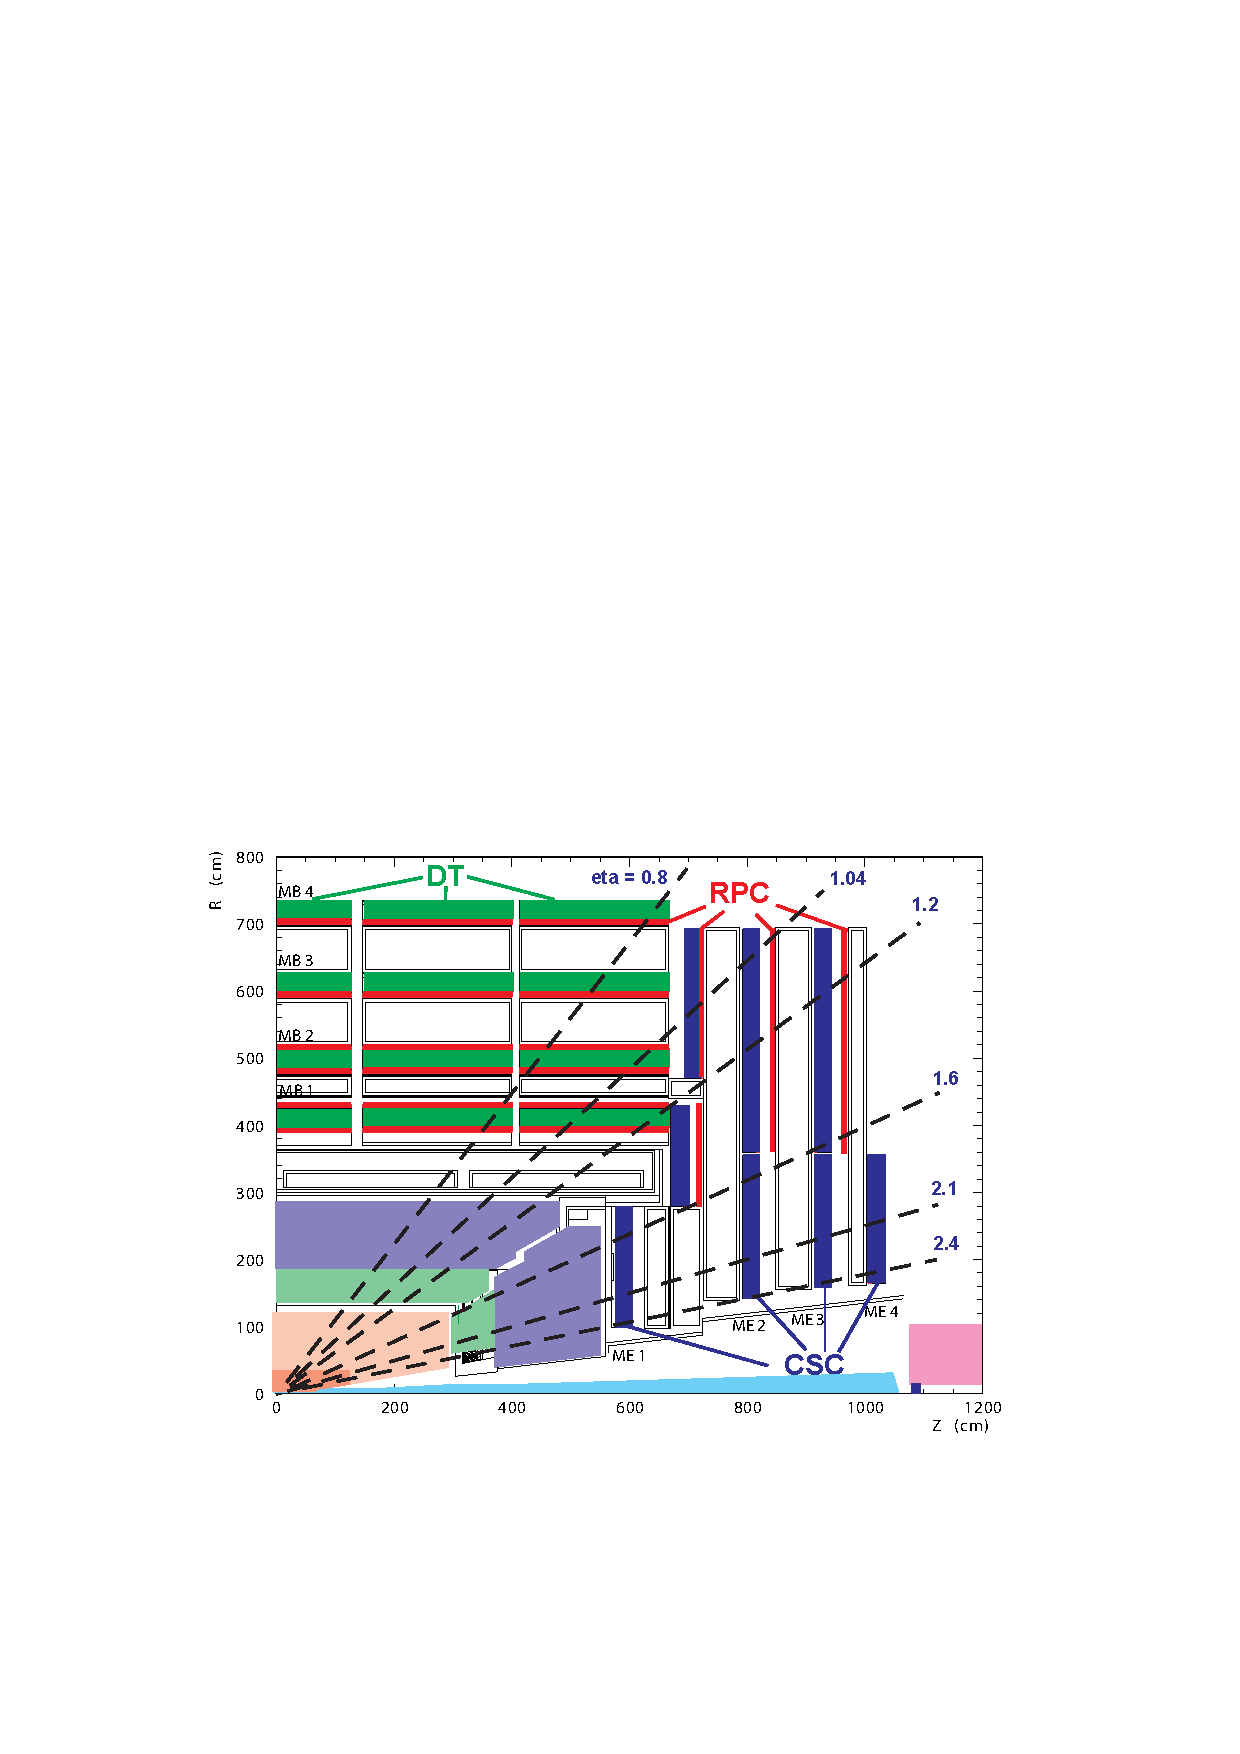
\includegraphics[width=0.9\columnwidth]{muon_system}
  \caption[Layout of one quarter of the CMS muon system]{Layout of one quarter of the CMS muon system. Four drift tube
  (DT, in light orange) stations are labeled MB (``muon barrel'') and the cathode strip chambers (CSC, in green) are
  labeled ME (``muon endcap''). Resistive plate chambers (RPC, in blue) are in both the barrel and the endcaps of CMS,
  where they are labeled RB and RE, respectively.}
  \label{fig:muon_system}
\end{figure}

The layout of the CMS muon system is shown in Figure~\ref{fig:muon_system}. It consists of the drift tubes (DT), cathode
strip chambers (CSC) and resistive plate chambers (RPC). The entire system surrounds the solenoid and covers the
pseudorapidity region of \abs\eta \num{<2.4}. Three different technologies are used in order to maximise the muon
triggering, identification and reconstruction efficiency in both barrel and endcap regions of the detector.

The drift tubes are located in the barrel region (\abs\eta \num{<1.2}). Consisting of four stations, they form
concentric cylinders around the beam line; there are \num{250} drift chambers with about \num{172000} sensitive wires in
total. When a muon passes through the volume, it knocks electrons off the atoms of the gas, which then follow the
electric field and reach the positively-charged wires, providing information on the muon's position. The chambers are
filled with the gas mixture of \SI{85}{\percent} $\textrm{Ar}$ and \SI{15}{\percent} $\textrm{CO}_2$, where the muon
drift time does not exceed \SI{380}{\ns}. Although this value is bigger than the typical bunch crossing time (\num{25}
or \SI{50}{\ns}), it is sufficient because of the small muon rate in this region.

In the endcaps, the cathode strip chambers cover the pseudorapidity region of \num{0.9} $<$\abs\eta\num{<2.4}. Each of
\num{468} CSCs is a trapezoidal multi-wire proportional chamber consisting of 6 gas gaps with a plane of radial cathode
strips and a plane of anode wires which are roughly perpendicular. A charged muon traversing each plane of a chamber
causes gas ionisation and a subsequent electron avalanche which produces a charge on the anode wire and an image charge
on the cathode strips. The gas used in CSCs is a mixture of $\textrm{Ar}$, $\textrm{CO}_2$ and $\textrm{CF}_4$.

The resistive plate chambers system is complementary to both DT and CSC systems, and is located in both barrel and
endcap regions (\abs\eta\num{<2.1}). RPCs also operate in avalanche mode with a gas mixture of C$_2$H$_2$F$_4$,
C$_4$H$_{10}$ and $\textrm{SF}_6$, and due to an excellent time resolution of about \SI{1}{\ns} they provide fast
information for triggering. The spacial resolution is, however, quite limited (\SI{\approx 1}{\cm}, compared to
\SI{\approx 100}{\micron} for DTs and CSCs). %http://arxiv.org/abs/1306.6905

\begin{figure}[htbp]
  \centering
  \leavevmode
  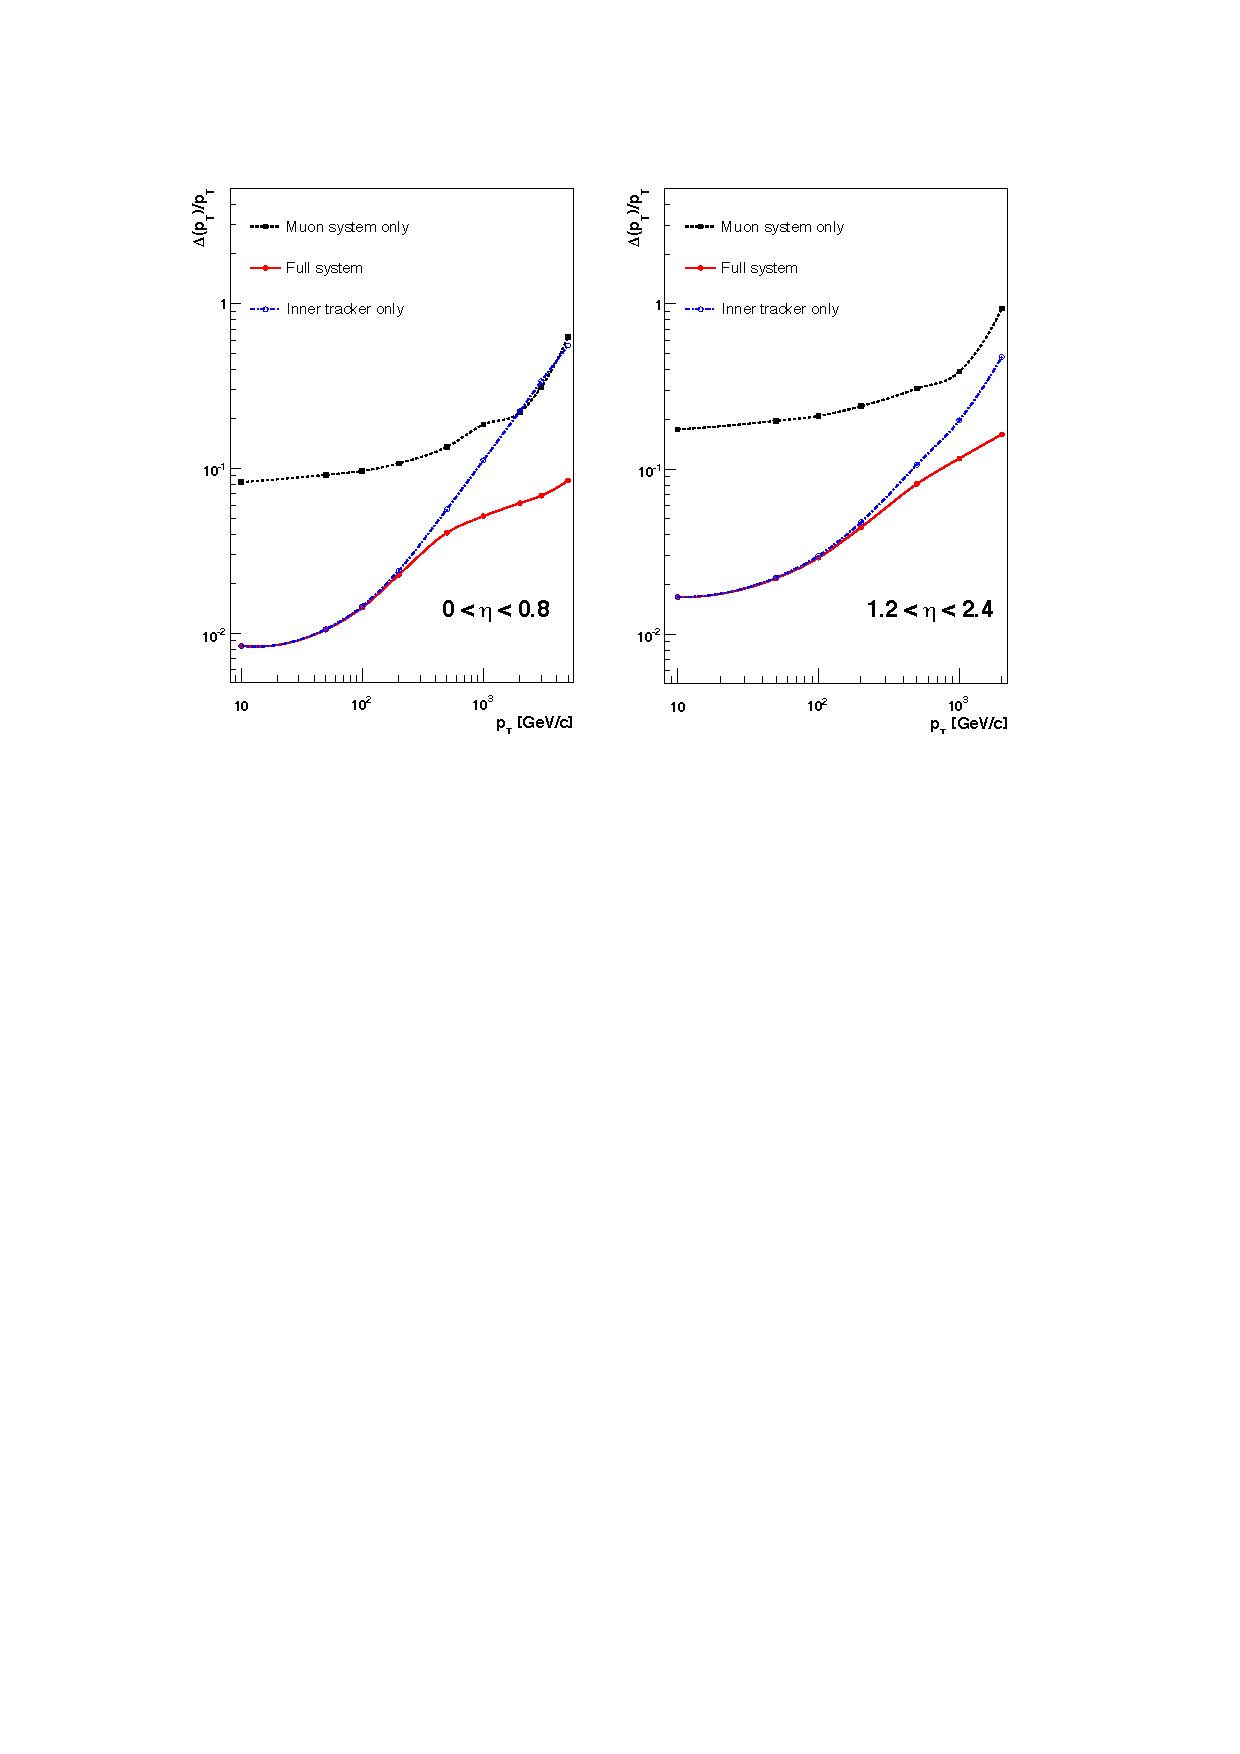
\includegraphics[width=\columnwidth]{muon_resolution}
  \caption[Muon transverse momentum resolution as a function of the transverse momentum]{Muon transverse momentum
  resolution as a function of the transverse momentum (\pt) using the muon system only (black), the inner tracking only
  (blue), and both (red), in regions of \abs\eta \num{<0.8} (left) and \num{1.2} $<$\abs\eta\num{<2.4} (right)
  \autocite{CMS}.}
  \label{fig:muon_resolution}
\end{figure}

The muon momentum is measured in both the tracker and the muon system.  As it can be seen on
Figure~\ref{fig:muon_resolution}, both sub-systems contribute to the momentum resolution at different \pt values. This
happens due to the difference in the magnetic field and detector technology. For low-\pt muons, the best momentum
resolution is obtained in the tracker, whereas in the high-\pt region the muon system provides a significant
improvement. Therefore, by using information from both the silicon tracker and the muon chambers (i.e.\ reconstructing
the ``global muon''), the momentum resolution is improved in the whole \pt region up to a \SI{\approx 1}{\TeV/c} level.

\subsection{Trigger and Data Acquisition}
\label{ss:trigger_daq}
At design LHC luminosity of $\calL = $ \SI{d34}{\cm^{-2} s^{-1}}, approximately \num{25} collisions are expected to
occur at each crossing of the proton bunches. The bunch spacing of \SI{25}{\ns} corresponds to a crossing rate of
\SI{40}{\mega\hertz}. Since every event produces \SI{\sim1}{\mega\byte} of raw data, it corresponds to a total data
production of \SI{40}{\tera\byte\per\second}. Attempting to store all of these data is clearly beyond the available
technology. Moreover, only a fraction of events contain hard scattering processes that are of interest, therefore an
effective trigger system had to be implemented.

The CMS trigger is a two-level system, consisting of two independent parts: the Level-1 (L1) trigger and the High Level
Trigger (HLT). The L1 trigger is a hardware system implemented in programmable electronics residing partly on detector,
and partly in the underground control room located at approximately \SI{90}{\metre} from the experimental cavern. The
maximum latency between the collision and the L1 accept decision received by front-end electronics is
\SI{3.2}{\micro\second}. During this amount of time, the complete event information is buffered in pipelined memories
on the detector. The only information used for the L1 trigger decision is that from the muon system and the calorimetry.
Since the reconstruction of tracks exceeds the time scale required for the L1 decision, the tracker information can't be
used. The L1 trigger reduces the event rate from \SI{\sim40}{\mega\hertz} to \SI{\sim100}{\kilo\hertz}, corresponding to
a data flow of about \SI{100}{\giga\byte\per\second}. These events are fed into the HLT system.

The High Level Trigger is a software system implemented in a single CPU farm, sometimes referred to as the ``Event
Filter Farm''. Having access to the full event information, customised algorithms of increasing complexity are used
which results in a highly flexible trigger system. The event rate is reduced down to \SI{\sim300}{\Hz}, with the final
data rate of approximately \SI{300}{\mega\byte\per\second} being stored on a large disk cache at the experimental site
(the Storage Manager) and later on transferred to CERN Tier 0 for further processing (see Section \ref{s:computing}).

Since the start of the LHC running, the operating conditions have been changing drastically. During the start-up year of
2010, the instantaneous luminosity went up from about \SI{d27}{\cm^{-2} s^{-1}} to approximately \SI{0.2d32}{\cm^{-2}
s^{-1}}. In 2011 the luminosity ramped up to a factor of \num{20} above that of 2010, reaching approximately
\SI{4d33}{\cm^{-2} s^{-1}}. This required a lot of continuous effort to control the trigger rates at reasonable level,
whilst also keeping its efficiency acceptable. In 2012 the luminosity was more stable, peaking at
\SI{\approx7.6d33}{\cm^{-2} s^{-1}} which is just a factor of 2 above the 2011 values. However, it still came as a
challenge because of the impact of pile-up. At a bunch spacing of \SI{50}{\ns} and increased centre of mass energy of
\SI{8}{\TeV}, the average number of pile-up vertices nearly doubled comparing to that in 2011, which required a major
CPU extension and implementation of sophisticated PU mitigation techniques at the HLT level. The author's contribution
to the HLT development of the trigger paths important for top physics is described in Chapter~\ref{c:service_work}.

\section{Computing}
\label{s:computing}
The vast amounts of data delivered by the CMS detector impose high requirements on the offline computing system. During
2010--2012 operation, CMS collected \SI{\sim10}{\peta\byte} of raw data per year. Including Monte Carlo simulation,
reconstructed data and analysis skims, the total annual amount of data essentially doubles. To handle the distributed
storage and processing of these data, not just for CMS but for the entire high energy physics community using the LHC, a
worldwide LHC computing grid (WLCG) has been put in place.

WLCG is a global collaboration of more than 150 computing centres in about 40 countries. The grid has a tiered
architecture, comprising 4 tiers with different resources and services. The first one, Tier 0, is based at CERN and is
responsible for data-taking. It accepts raw data from the data acquisition system and repacks it into primary datasets
according to the trigger information. The raw data are archived to tape, and is also prompt-reconstructed (within 48
hours) before being distributed to the Tier 1 (T1) centres around the world. There are 8 T1 sites based at large
national laboratories in collaborating countries (e.g.\ Rutherford Appleton Laboratory in the UK and Fermi National
Accelerator Laboratory in the US). Each of the T1 centres is used for large-scale centrally organised data-processing
activities. The data are then distributed in a reduced format (see Section~\ref{ss:edm}) to a more numerous set of Tier
2 centres, typically located at collaborating universities. Each of these centres is used for the grid-based analysis
and Monte Carlo simulation for the whole experiment, as well as local services for groups maintaining them. The last
stage of computing system, Tier 3, is meant solely for the local institution's user analysis.

\subsection{Event Data Model}
\label{ss:edm}
At the heart of the CMS Event Data Model lies the concept of an event, which is physically a result of a single
collision in the LHC. From a software point of view, the event is a \Cplusplus object container storing raw data from a
single readout of detector electronics (e.g.\ hits in various sub-detectors), as well as reconstructed data which is
based on this information, such as tracks, clusters and physics objects. All these \Cplusplus objects are stored in ROOT
format \autocite{ROOT}.

The EDM makes use of three main data formats, based on different levels of detail and precision:
\begin{itemize}
  \item RAW format, containing full information from the detector as well as L1 and HLT trigger decisions, with an event
  size of \SI{\sim1.5}{\mega\byte}.
  \item RECO (reconstructed data) format, which is obtained from raw data by application of pattern recognition and
  compression algorithms. This data includes reconstructed detector hits, clusters and physics objects (electrons,
  muons, etc.). The typical event size is \SI{\sim250}{\kilo\byte}.
  \item AOD (Analysis Oriented Data) format, produced by filtering the RECO data from the reconstructed detector
  objects, leaving just the high-level physics objects required for analysis. The event size is reduced down to
  \SI{\sim50}{\kilo\byte}.
\end{itemize}

The RECO and AOD data are analysis-ready data formats, produced centrally and used by many physics analysis groups.
However, further simplification of the data is also a common practice. By transforming the \Cplusplus objects produced
by CMS software into plain basic types or vectors of them, only including the analysis-specific content, the event size
can be reduced down to \SI{\sim3}{\kilo\byte} level depending on the needs of a particular analysis. This data format is
often referred to as private ``ntuples'', and it requires specific analysis software capable of restructuring the data
into user-defined classes. By following this approach, the analysis can be run locally and generally much faster than
processing the RECO or AOD data. However, it requires ``ntuplising'' these data every time when new centrally-recommended
physics objects or corrections are produced.

\subsection{Analysis Software}
\label{ss:analysis_software}
Both of the analyses described in this thesis use the CMS software framework (CMSSW \autocite{CMSSW}), as well as
Bristol Analysis Tools (BAT \autocite{BAT}). The differential cross section analysis also uses an additional level of
python scripts for post-processing \autocite{DailyPythonScripts}.

CMSSW is the key CMS software framework built around the Event Data Model (see Section~\ref{ss:edm}). The framework is
essential for purposes of Monte Carlo simulation, detector calibration and alignment, as well as data reconstruction
and analysis. CMSSW has a modular architecture, consisting of one configurable executable (cmsRun) and a large set of
plug-in modules that contain all the code needed for event processing (reconstruction algorithms, calibration, etc.).
Different versions of CMSSW were used for different analyses: 

\begin{itemize}
  \item CMSSW\underline{\hspace{1ex}}4\underline{\hspace{1ex}}2\underline{\hspace{1ex}}8 for the top mass analysis on 2011 data;
  \item CMSSW\underline{\hspace{1ex}}4\underline{\hspace{1ex}}4\underline{\hspace{1ex}}4 for the missing transverse energy analysis on 2011 data;
  \item CMSSW\underline{\hspace{1ex}}5\underline{\hspace{1ex}}3\underline{\hspace{1ex}}9 for the top cross pair cross section analysis on 2012 data.
\end{itemize}

Corresponding versions were used to produce ntuples for processing by BAT, which was used to read the data, apply
selections, calculate high-level variables and to create various histograms of distributions. BAT was originally started
in 2010 by \L{}ukasz Kreczko for the needs of the Bristol top group, later on also developed by the author and other
researchers from Bristol and affiliated top groups. Like CMSSW, this framework has a modular structure, with its classes
falling in four main categories:

\begin{itemize}
  \item readers, for translating plain data types from ROOT files into \Cplusplus objects;
  \item RECO objects, i.e.\ output of the readers (physical objects like leptons, jets and its collections);
  \item selections, for application of event selections;
  \item analysers for creating histograms, applying selections, algorithms, and filling histograms.
\end{itemize}

All analysers are independent from each other, making the analysis chain stable and reliable. The final set of python
scripts is used to prepare the histograms, perform fitting and unfolding procedures (in case of cross section analysis),
and producing final tables and plots. Rootpy package \autocite{rootpy} was used to access ROOT libraries in python
interface, and matplotlib \autocite{matplotlib} was used to create plots.

\section{Monte Carlo Simulation}
\label{s:MC_simulation}
To develop and test any analysis technique in modern particle physics, simulated events from Monte Carlo (MC) generators
as well as a working simulation model of the detector are inevitably needed. All current theoretical knowledge of the
Standard Model processes is incorporated in Monte Carlo simulation, and can be validated by direct comparison of the
simulated events with real data. Any deviations may indicate the signs of new physics processes, which are also
simulated according to various BSM physics models. On the other hand, these deviations can also be caused by
deficiencies in the simulation process. Therefore, adequate and robust MC simulation is crucial for both precision
measurements and searches for new physics.

Different MC simulation techniques exist and can be used in various MC generators. In this section, the basic concepts
of MC simulation are introduced. All the event generators exploited in this thesis as well as different MC tunes used
for evaluation of theoretical uncertainties are briefly described. Additionally, the \GEANTfour-based
\autocite{GEANT4} simulation of the CMS detector is mentioned.

\subsection{Generation of hadron collision events}
\label{ss:hadron_collisions_simulation}

Simulation of hadron collision events is a rather complicated process. It is usually factorised into the following
steps, schematically illustrated in Figure~\ref{fig:MC_simulation_graphics}:

\begin{enumerate}[label=\textbullet]
  \item incoming hadrons (protons);
  \item hard scattering of partons;
  %\item boson radiation (\Z, \photon, \cPg);
  \item parton showers;
  \item hadronisation of partons and hadron decays;
  \item underlying event.
\end{enumerate}

\begin{figure}[htbp]
  \centering
  \leavevmode
  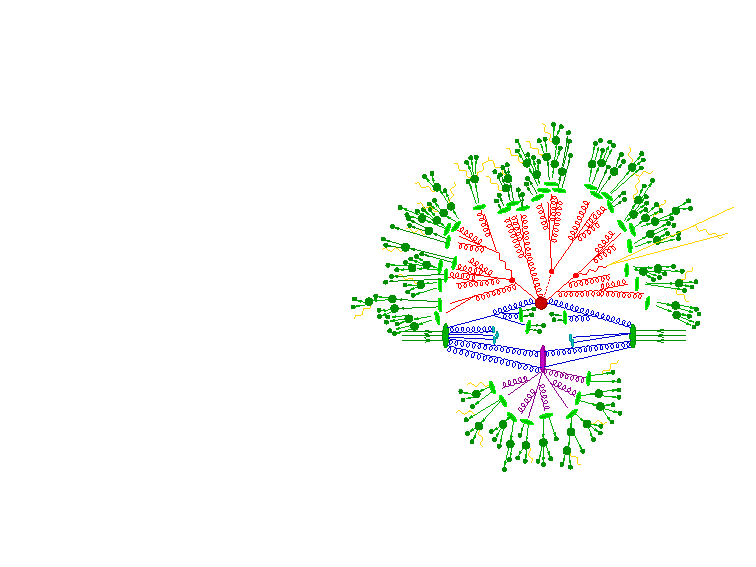
\includegraphics[width=0.7\columnwidth]{MC_simulation_graphics}
  \caption[Schematic overview of a hadron collision process]{Schematic overview of a hadron collision process
  \autocite{Hoeche_slides}}
  \label{fig:MC_simulation_graphics}
\end{figure}

The simulation of hadron collisions makes use of the factorisation between the short-distance hard scattering process
and long-distance soft interactions described by parton distribution functions, as shown in
Section~\ref{ss:ttbar_cross_section}. In matrix-element MC generators such as \MADGRAPH, the hard scattering process is
described by calculating the tree-level matrix elements and including higher-order corrections, i.e.\ additional partons
in the final state. The generator produces all possible Feynman diagrams for a renormalisable Langrangian-based model,
and generates its matrix elements at the tree level, performing the integration over all phase-space. This calculation
is then used to produce the cross section of various processes and subprocesses, as well as partons and parton decays.

Partons from matrix element calculations are then matched to parton showers. Accelerated coloured partons emit QCD
radiation in the form of gluons, similarly to QED radiation emitted by accelerated electric charges. But since gluons
also carry a colour charge, they emit further radiation, which results in parton showering. It is convenient to describe
it in terms of the initial state radiation (ISR), which refers to the radiation of incoming partons, and the final state
raditation (FSR), i.e.\ radiation of outgoing partons. Theoretically, parton showers can be regarded as higher-order
corrections to the hard scattering process. However, precise calculation of these corrections is not feasible, therefore
an approximation scheme is used, based on QCD evolution equations first described by Dokshitzer, Gribov, Lipatov,
Altarelli and Parisi (DGLAP) \autocite{Dokshitzer, Gribov_Lipatov, Altarelli_Parisi}.

After the parton showering is modelled, colour-neutral hadrons have to be formed in the hadronisation process according
to the colour confinement, as described in Section~\ref{ss:QCD_theory}. The most widely used hadronisation model
(implemented in \PYTHIA generator) is the Lund string model, where gluons are split into \qqbar pairs and then turned
into hadrons via the string fragmentation model \autocite{Lund_model}.

% Another hadronisation model is based on cluster fragmentation, where colourless clusters are formed from quarks and
% gluons with low invariant masses, which then are turned into clusters. (HERWIG)

Finally, apart from the hard scattering process, it is also important to model all the additional activity in
proton-proton collisions, which is referred to as underlying event activity \autocite{underlying_event}. This activity
includes multiple interactions of the remaining partons in hadron collisions, and beam remnants which do not participate
in the hard scattering. Both the multiple parton interactions and the beam remnants carry a colour charge and produce
additional soft hadrons. The colour charges from all the activity in the event, including the hard scattering process,
ISR and FSR, beam remnants and multiple parton interactions can interact in a very non-trivial manner. This leads to
additional uncertainty called colour reconnection \autocite{colour_reconnection}, which also affects the whole
hadronisation process and may result in biased precision measurements. To account for all known hadronisation and
underlying event effects, phenomenological models with free parameters need to be tuned to data. Different tunes can
then be used to estimate the systematic uncertainties arising from imperfect understanding of these effects.

One of the most significant systematic uncertainties can arise from the procedure of matching the matrix elements to
parton showers. There is a certain threshold for partons transverse momenta from matrix element calculations to be
matched with parton showers, often referred to as ME-PS threshold. To estimate the systematic uncertainty arising from
it, additional MC samples are generated with the varied value of the threshold. In this thesis, this procedure was
performed for signal \ttjets and background \WpJets and \ZpJets samples. Similarly, the systematic effect of the choice
of factorisation scale $Q^2$ (described in Section~\ref{ss:top_production}) is also be determined.

\subsection{Monte Carlo event generators}
\label{ss:MC_generators}
In the analyses presented in this thesis, all physics processes were generated with a set of different MC generators,
including \MADGRAPH \autocite{MadGraph}, \PYTHIA \autocite{Pythia,Pythia6.4}, \MCATNLO \autocite{MCatNLO}, and \POWHEG
\autocite{POWHEG}. The performance of MC generators is usually optimised for one or more of the simulation steps
described above, therefore two or more generators are often used in combination. For example, the nominal \ttbar signal
samples used in this thesis are modelled with \MADGRAPH and \PYTHIA. Standalone generators can also be used for
modelling theory systematic effects, which is also exploited in this thesis.

%A supplementary package (\TAUOLA \autocite{TAUOLA}) was used for the tau lepton decay description.

\begin{description}[wide=\parindent, style=standard, labelsep=0pt]
\item [\MADGRAPH] \autocite{MadGraph} is a multi-purpose matrix-element Monte Carlo event generator. It automatically
generates matrix elements for decays and $2 \rightarrow n$ scatterings. The matching of matrix elements to parton
showers is performed according to the so-called MLM prescription \autocite{MLM} if a parton-jet pair satisfies a certain
$\Delta R$ separation criterion. If no or more than one matched jets are found, events are rejected. As it was
mentioned, there is also a certain transverse momentum threshold requirement for the partons to be considered in the
matching. Default values as well as variations used to estimate the systematic effect of the matching threshold can be
found in Table~\ref{tab:systematic_mc_variations}.

\item [\PYTHIA] \autocite{Pythia,Pythia6.4} is one of the most widely used MC generators in high energy physics. It is a
standard tool used for simulation of initial protons fragmentation, multi-particle production, quark and gluon
hadronisation, beam remnants and the underlying event. In this work, \PYTHIA is used to generate QCD multi-jet
production, and to simulate the underlying event on top of other generators providing partons from hard processes.

\item [\MCATNLO] \autocite{MCatNLO} is a parton shower MC generator providing next-to-leading order (NLO) corrections
for a simulated process. It represents a major improvement in precision and accuracy of physics simulations comparing to
leading order (LO) generators like \PYTHIA. An NLO implementation can handle additional partons in the final state
coming from the hard scattering, which is not possible with LO calculations. Therefore it includes additional dynamic
features, giving a major advantage for heavy flavour physics.

\item [\POWHEG] (Positive Weight Hardest Emission Generator) \autocite{POWHEG} also works at NLO precision. Its main
difference to \MCATNLO generator lies in the order of process generation: \POWHEG initially generates the hardest
radiation. This technique allows to avoid double-counting coming from subsequent radiation which may happen with
\MCATNLO method when matching QCD NLO calculations with parton showers.
%http://theory.fnal.gov/seminars/slides/2008/COleari.pdf

\end{description}

\subsection{CMS detector simulation}
\label{ss:detector_simulation}

Detector simulation is an essential final step on top of the full physics simulation of proton-proton collisions. All
generated particles resulting from these collisions are propagated to the simulated layers of the detector so that their
interaction with the detector material and detector response can also be modelled. The CMS simulation is based on the
\GEANTfour (GEometry ANd Tracking \autocite{GEANT4}) package, which is implemented in CMS software \CMSSW
\autocite{CMSSW}. This package fully recreates the geometry of the detector, including all its subsystems as well as a
detailed map of the magnetic field.

In general, the simulation procedure includes modelling of the following steps:
\begin{enumerate}[label=\textbullet]
  \item interaction region;
  \item particles traversing all the layers of the detector and the interaction processes;
  \item multiple interactions per beam crossing (pile-up) and event overlay effects;
  \item digital readout of the detector (digitisation).
\end{enumerate}
%https://twiki.cern.ch/twiki/bin/view/CMSPublic/SWGuideSimulation

The data stream generated with this process is very similar to the output of the real detector, although naturally in
addition to reconstructed objects, generated events also include collections of generated objects, allowing users to
access the Monte Carlo truth information, which is essential for any particle physics analysis.

\newpage
\section{Object Reconstruction}
\label{s:object_reconstruction}
Most CMS analyses, including the ones described in this thesis, adopt a reconstruction technique called Particle Flow
(PF) \autocite{PF}. This algorithm is used to obtain a global event description at the level of individually
reconstructed particles by means of combining information coming from all sub-detector systems. The ultimate goal is to
determine type, energy and momentum of all the particles in the event with highest possible precision and in the most
optimal way. The types of these particles include electrons, muons, charged hadrons, neutral hadrons and photons. All
these particles are then used to reconstruct jets (Section~\ref{ss:jet_reconstruction}), missing transverse energy
(Section~\ref{ss:electron_reconstruction}) and tau leptons from their decay products.

\subsection{Electron reconstruction}
\label{ss:electron_reconstruction}
The reconstruction of the \ttbar pair with an electron in the final state (see
Section~\ref{fig:ttbar_semileptonic_decay}) imposes strict requirements on the electron identification and its
energy-momentum measurement, precision of which is of major importance for both top mass and
\ttbar cross section measurements.

Although the CMS detector is equipped with highly accurate ECAL and tracker systems, electron identification and
reconstruction is still a challenging task due to the large amount of tracker material (see Section~\ref{ss:tracker}).
This results in significant Bremsstrahlung photon emission, which often causes an ECAL energy deposit to be widely
spread in the azimuthal direction because of the high magnetic field. Therefore, dedicated algorithms were developed in
order to collect all Bremsstrahlung energy deposits in the calorimeter (Bremsstrahlung recovery), and also to take into
account the kinks in the electron trajectory caused by photon emission.

Electron reconstruction in CMS has the following distinct stages: seeding; track finding; pre-identification;
Bremsstrahlung recovery; track-cluster linking; and final identification. Historically, the original seeding algorithm
was designed and optimised for isolated high-\pt electrons. This approach starts from ECAL clusters, and therefore is
called the ``ECAL-driven'' seeding. It is based on the property of ECAL energy deposits to have narrow width in the
$\eta$ coordinate, and to be widely spread in $\phi$ (azimuthal direction) as mentioned above. The electron and all the
associated Bremsstrahlung energy deposits form a single ``super-cluster'', and the ability to correctly identify it
affects the overall performance of this method. Super-clusters are then matched to pairs or triplets of hits in the
inner tracker layers, forming the track seeds on which the electron tracks are built upon.
%Only super-clusters with transverse energy above \SI{4}{\GeV} are taken into account.

The performance of the ECAL-driven method is not very well suited for non-isolated and low-\pt electrons. This occurs
mainly due to the fact that the super-cluster position and energy can be highly biased by the impact of overlapping
particles, especially if the electron happens to be within a jet and therefore non-isolated. Also, high track
multiplicity complicates the backward propagation from a super-cluster, because it can be consistent with a number of
track seeds corresponding to other particles.

% To minimise the number of these fake seeds, the ratio between the HCAL and ECAL energy deposits ($H/E$) is required to
% be smaller than \num{0.15}. The HCAL towers used in the calculation of this ratio are taken within a cone of $\DR = 0.3$
% behind the super-cluster position. Although this helps to keep the fake seed rate under control, the efficiency for
% non-isolated electrons becomes rather limited. As for the low-\pt electrons, the wider azimuthal spread of
% Bremsstrahlung photons leads to poorer reconstruction of the super-cluster, biasing its position and therefore
% preventing the efficient matching with a track seed.

Within the particle flow method, efficient reconstruction of non-isolated and low-\pt electrons is particularly
important since it affects the reconstruction of jets and missing transverse energy. Therefore, a different
(``tracker-driven'') seeding algorithm is used, which starts from reconstruction of tracks. The baseline of the CMS
track reconstruction is the Kalman filter (KF) \autocite{KF}, which is a linear least-squares estimator based solely on
Gaussian probability density functions. It is particularly suitable for muon reconstruction, since the interaction of
muons with matter is dominated by multiple Coulomb scattering, which is well modelled by Gaussian fluctuations. However,
this approach usually fails for electrons because Bremsstrahlung photon emission is highly non-Gaussian. To accommodate
the resulting kinks in the electron trajectory, the Gaussian-Sum Filter (GSF) \autocite{GSF} is used, which is
essentially a non-linear generalisation of the Kalman Filter. In this method, Bremsstrahlung energy loss is modelled by
a Gaussian mixture, therefore the GSF track fit provides a better estimate for the inner and outer track momentum
compared to the KF algorithm. The downside of this approach is its high CPU usage, which means it can be run only on a
limited number of seeds.

The GSF tracks are reconstructed upon all ECAL-driven seeds. In the case of ``tracker-driven'' seeds, a
pre-identification based on high-purity KF tracks has been adopted. This procedure starts with the tracks reconstructed
with very tight criteria, thus decreasing the fake rate yet compromising on tracking efficiency. Then an
iterative-tracking strategy is carried out by means of removing hits unambiguously assigned to tracks from the previous
iteration, and also progressively relaxing track seeding criteria. This approach leads to both high efficiency and low
fake rate, which is crucial for low-\pt and non-isolated electrons.

In the next step, track-cluster matching is performed. In the case where an electron has negligible Bremsstrahlung
emission, the track is well reconstructed with the KF algorithm all the way to the ECAL internal surface, where the
closest cluster is matched to the track. The corresponding cluster energy is compared with the track momentum, and if
the ratio ($E/p$) is close to unity, the track is selected. On the contrary, if the electron experiences a significant
Bremsstrahlung emission, other track characteristics are used. In this case a selection based on the number of hits in
the tracker and the $\chi^2_\textrm{KF}$ of the KF fit is applied before running a GSF refit. Finally, the number of
hits, the GSF refit $\chi^2_\textrm{GSF}$, $\chi^2_\textrm{KF}/\chi^2_\textrm{GSF}$ ratio, the energy loss measured by
the track and the quality of the ECAL cluster-track matching are fed into a multivariate analysis using a Boosted
Decision Tree (BDT) estimator.

Both tracker-driven and ECAL-driven seeds are used to obtain the GSF track collection of electron candidates. In the
particle flow algorithm, it is necessary to link both electron and Bremsstrahlung energy deposits to the GSF track. A
super-cluster is linked to a track if the extrapolated position from the outermost tracker measurement is within the
boundaries of one of the ECAL cells at the expected depth of the electron shower maximum. The preshower-ECAL and
ECAL-HCAL links are made in a similar way.

Another important particle flow procedure, also driven by GSF tracks, is Bremsstrahlung recovery. In order to
reconstruct an electron with correctly assigned energy and momentum, it is crucial to identify all energy deposits from
Bremsstrahlung photons, thus forming a super-cluster. This procedure is carried out for each tracker layer by computing
a straight-line extrapolation tangent to the track, up to the calorimeter. To determine a Bremsstrahlung photon,
track-cluster linking is performed as described above. To limit the charged hadron contamination, clusters already
assigned to KF tracks are not included in the calculation.

% Also, the distance in $\eta$ coordinate between the extrapolation and the cluster is required to be smaller than
% \num{0.015}, which helps to reduce the neutral particle background.

\subsubsection{Electron identification}
\label{sss:electron_id}

Electron reconstruction in CMS is based on a characteristic signature that electrons leave in the tracker and
calorimetry systems. However, other objects like charged hadrons, jets or photon conversions can produce very similar
signatures and therefore may be reconstructed as electrons. Therefore, in order to distinguish these ``fake'' electrons
from ``real'' ones, a further selection has to be applied. This procedure is referred to as electron identification (or
electron ID).

Initially, the electron identification is performed at the final stage of the electron reconstruction process. The
working points of the cuts applied are selected to be loose enough in order to satisfy the requirements of most CMS
analyses. Afterwards, more specific (tighter) ID cuts are applied for each individual analysis, defining the working
point in the trade-off between selection efficiency and contamination from fakes. This will be discussed separately in
the selection description for each analysis in corresponding chapters.

Different algorithms are used for electron identification at different stages of physics analysis. These algorithms use
information from both the tracker and calorimeter systems combined in different ways, including the track quality
variables, ECAL shower shape variables, track and super-cluster mathcing variables and Bremsstrahlung variables. The
full list of variables used by electron ID algorithms described below is given in Table~\ref{tab:electron_ID_variables}.

% \begin{itemize}
%   \item $H/E$, i.e.\ the ratio of the hadronic energy associated with the electron candidate to the super-cluster
%   energy. The hadronic energy is found by summing the HCAL towers in a cone of radius $\Delta R = 0.15$, centred at the
%   super-cluster position;
%   \item $\Delta\eta_{\text{in}}$, i.e.\ the difference in $\eta$ between the extrapolated track position and $\eta$ of
%   the super-cluster;
%   \item $\Delta\phi_{\text{in}}$, i.e.\ the difference in $\phi$ between the extrapolated track position and $\phi$ of
%   the super-cluster;
%   % \item $\sigma_{i\eta, i\eta}$, i.e.\ a cluster shape of the electron energy in a $5\times5$ block of crystals around the
%   % seed crystal (the one with the highest energy) \autocite{electron_reconstruction}:
%   \item $\sigma^2_{i\eta, i\eta}$, i.e.\ the cluster shape variable that gives a measure of the width of the cluster in
%   $\eta$, using the distribution of energy in a $5\times5$ block of crystals around the seed crystal (the one with the
%   highest energy) \autocite{electron_reconstruction}:
%   \begin{equation}
%   \label{eq:cluster_shape}
%     \sigma^2_{i\eta, i\eta} = \sum_{5\times5 \text{ crystals}} \left(\eta_i - \eta_\text{seed cluster}\right)^2
%     \frac{E_i}{E_{\text{seed cluster}}}
%   \end{equation}
% \end{itemize}

\newpage
\begin{longtable}{| p{.2\textwidth} | p{.75\textwidth} |} 
  \caption{Variables used in electron identification algorithms} \label{tab:electron_ID_variables} \\
  \toprule
  \textbf{Variable} &  \multicolumn{1}{c|}{\textbf{Description}} \\    
  \midrule
  \multicolumn{2}{|c|}{\textit{Track quality variables}} \\
  \midrule
  \pt & Transverse momentum of the GSF track \\
  \midrule
  $\eta$ & Pseudorapidity of the GSF track \\
  \midrule
  GSF $\sigma_{p_\text{T}}/p_\text{T}$ & Transverse momentum resolution of the GSF track\\
  \midrule
  \#hits$_\text{KF}$ & Number of reconstructed KF track hits\\
  \midrule
  $\chi^2_\textrm{GSF}$ and $\chi^2_\textrm{KF}$ & GSF and KF goodness-of-fits\\
  \midrule

  \multicolumn{2}{|c|}{\textit{ECAL shower variables}} \\
  \midrule
  $\sigma^2_{i\eta, i\eta}$ & Cluster shape variable that gives a measure of the width of the cluster in $\eta$, using the distribution of energy in a $5\times5$ block of crystals around the seed crystal (the one with the highest energy) \autocite{electron_reconstruction}:\newline
  $\sigma^2_{i\eta, i\eta} = \sum_{5\times5 \text{ crystals}} \left(\eta_i - \eta_\text{seed cluster}\right)^2 E_i / E_{\text{seed cluster}}$ \\
  \midrule
  $\sigma^2_{i\phi, i\phi}$ & Cluster shape in $\phi$\\
  \midrule
  $\eta_\text{SC}$ ($\phi_\text{SC}$) & Width of the super-cluster in $\eta$ ($\phi$)\\
  \midrule
  $1-E_{1\times 5}/E_{5\times 5}$ & $E_{1\times 5}$ is the energy in the central $1\times 5$ strip of the
  $5\times 5$ electron cluster and $E_{5\times 5}$ its total energy\\
  \midrule
  $E_{3\times 3}/E_\text{SC, raw}$ & Ratio of the energy of a cluster of $3\times 3$ to the
  uncorrected (raw) energy of the super-cluster\\
  \midrule
  $E_\text{PS}/E_\text{SC, raw}$ & Ratio of the energy in the preshower detector to the raw
  super-cluster energy (only in the endcap region)\\ 
  \midrule

  \multicolumn{2}{|c|}{\textit{Longitudinal shower shape variables}} \\
  \midrule
  $H/E$ & Ratio of the hadronic energy associated with the electron candidate to the super-cluster energy. The hadronic energy is found by summing the HCAL towers in a cone of radius $\Delta R = 0.15$, centred at the super-cluster position\\
  \midrule
  $H/(H+E_\text{e})$ & Hadron fraction of the shower, where $H$ is the energy of the hadron cluster linked to
  the GSF track\\
  \midrule

  \caption{Variables used in electron identification algorithms (continued)} \\
  \midrule


  \multicolumn{2}{|c|}{\textit{Track/super-cluster matching variables}} \\
  \midrule
  $\Delta\eta_{\text{in}}$ ($\Delta\phi_{\text{in}}$) & Distance in $\eta$ ($\phi$) between the super-cluster
  position and the extrapolated track position \\
  \midrule
  $\Delta\eta_{vtx}$ ($\Delta\phi_{vtx}$) & Distance in $\eta$ ($\phi$) between the super-cluster
  position and the position of the GSF track at vertex \\
  % \midrule
  % $E_\text{SC}/p_\text{T}$ & Ratio of the super-cluster energy to the initial track momentum \\
  \midrule
  $(E_\text{e}+\sum E_\gamma)/p_\text{in}$ & Ratio of the super-cluster energy to the inner track
  momentum\\
  \midrule
  $E_\text{e}/p_\text{out}$ & Ratio of the electron cluster energy to the outer track momentum\\
  \midrule
  $1/E_\text{SC} - 1/p_\text{T}$ & Difference between inverse super-cluster energy and inverse
  track\newline momentum\\
  \midrule

  \multicolumn{2}{|c|}{\textit{Bremsstrahlung variables}} \\
  \midrule
  $f_\text{brem}$ & Measured bremsstrahlung fraction, defined as:
  $f_\text{brem} = (p_\text{in}-p_\text{out})/p_\text{in}$, where $p_\text{in}$ is the initial track momentum at the vertex and $p_\text{out}$ is the track momentum at the last hit\\
  \midrule
  $\sum E_\gamma/(p_\text{in}-p_\text{out})$ & Ratio between the Bremsstrahlung photon energy as measured by
  ECAL and by the tracker\\
  \midrule
  $EarlyBrem$ & Flag of $(E_\text{e}+\sum E_\gamma)>p_\text{in}$ inequality, corresponding to an electron
  emitting an ``early'' Bremsstrahlung photon, i.e.\ before it has crossed at least three tracker layers\\
  \midrule
  $LateBrem$ & Flag of $E_\text{e}>p_\text{out}$ inequality, corresponding to an electron emitting a ``late''
  Bremsstrahlung electron, when the ECAL clustering is not able to disentangle the overlapping electron and photon
  showers\\

  \bottomrule
\end{longtable}

\newpage


There are several electron identification algorithms used by various CMS analyses, and four of them are used in the
analyses described in this thesis: simple cut-based (SCB ID), cuts in categories (CiC ID), particle flow (PF ID) and
multivariate analysis (MVA ID).

\begin{description}[wide=\parindent]
  \item[Simple cut-based ID] \autocite{SCB_ID} is used in the High Level Trigger, and therefore has to be as simple,
fast and robust as possible. This algorithm only uses a limite number electron ID variables shown in
Table~\ref{tab:electron_ID_variables}, including $H/E$ ratio, $\Delta\eta_{\text{in}}$ and $\Delta\phi_{\text{in}}$
matching variables, cluster shape variables and isolation variables (to be described in the next section). Although this
identification method has an advantage of its simplicity, it does not show the best signal efficiency and background
rejection.

 \item[Cuts in categories ID] \autocite{CiC_ID} is one of the more complex methods, exploiting the categorisation of
electrons. It is optimised to select electrons from different sources (W, Z and J/$\psi$ decays) and reject fakes from
jets or conversions. In order to achieve higher efficiency, electron candidates are split into categories with different
signal to background ratio, allowing for better tuning of the working points of the cuts. The categories are formed by
selection based on the mentioned ID variables, as well as isolation and conversion rejection variables; these are
discussed in Section~\ref{sss:electron_isolation} and Section~\ref{sss:photon_conversions}, respectively.

% The first step in categorisation is done by division between barrel and endcap regions of the detector. Since the
% properties of both the tracker and calorimetry systems differ significantly in these two regions, different cuts are
% applied.

% Later categorization is performed using the Bremsstrahlung variables and electron transverse energy. In each category,
% the selection is performed on the basic ID variables already mentioned above for the simple cut-based identification. On
% top of these variables, isolation and conversion rejection variables are also used; these are discussed in
% Section~\ref{sss:electron_isolation} and Section~\ref{sss:photon_conversions}, respectively.

%The second step is based on the following observables:
% \begin{itemize}
%   \item $f_\text{brem}$, or measured bremsstrahlung fraction, defined as:
%   \begin{equation}
%   \label{eq:fbrem}
%     f_\text{brem} = \frac{p_\text{in}-p_\text{out}}{p_\text{in}}
%   \end{equation}
%   where $p_\text{in}$ is the initial track momentum at the vertex and $p_\text{out}$ is the track momentum at the last
%   hit;
%   \item $E/p$, which is the ratio of the super-cluster energy and the initial track momentum.
% \end{itemize}

% consider showing the supporting plot, but not found in vector.

% Three categories of electron candidates are distinguished:
% \begin{itemize}
%   \item ``Low-Brem'': $0.9 < E/p < 1.2 - f_\text{brem} < 0.12$ (barrel), $0.82 < E/p < 1.22 - f_\text{brem} < 0.2$
%   (endcap), the fake-like region with high number of both real and fake electrons;
%   \item ``Bremming'': $0.9 < E/p < 1.2 - f_\text{brem} > 0.12$ (barrel), $0.82 < E/p < 1.22 - f_\text{brem} > 0.2$
%   (endcap), the electrons-like region with a little contamination from fakes;
%   \item ``Bad-Track'': remaining regions with a low number of real electrons.
% \end{itemize}

% The third and the final step in categorisation is based simply on the electron transverse energy, with the lower
% threshold taken as \SI{10}{\GeV}. 

The cuts within CiC ID are applied in order to maximise the signal to background ratio. Depending on the needs of
different analyses, nine levels of cut severity are implemented: \textit{VeryLoose, Loose, Medium, Tight, SuperTight,
HyperTight(1-4)}. Each step decreases the fake rate by about a factor of two for electrons with \ET$>$ \SI{20}{\GeV}
\autocite{CiC_ID}. The CiC ID is used as a primary electron identification method in the top quark mass analysis
(Chapter~\ref{c:top_mass_analysis}).

 \item[Particle flow ID] \autocite{PF} is the final step of the particle flow electron reconstruction. Following the
particle flow concept, it uses information from all the CMS sub-detectors obtained in previous reconstruction steps to
build new observables for electron identification. The variables shown in Table~\ref{tab:electron_ID_variables} are
combined into a single discriminator by a multivariate analysis technique (BDT method), which has been trained on signal
and background Monte Carlo samples. PF ID is a relatively loose identification method, since it has to satisfy the needs
of all analyses using particle flow collections.

% \begin{itemize}
%   \item \pt and $\eta$ of the GSF track;
%   \item GSF $\sigma_{p_\text{T}}/p_\text{T}$, transverse momentum resolution of the GSF track;
%   \item \#hits$_\text{KF}$, number of reconstructed KF track hits;
%   \item $\chi^2_\textrm{GSF}$ and $\chi^2_\textrm{KF}$, GSF and KF goodness-of-fits;
%   \item $\Delta\eta$: distance in $\eta$ between the position of the cluster and the extrapolated position of the
%   GSF track;
%   \item $\sigma_{\eta\eta}$, cluster shape (see Table~\ref{tab:electron_ID_variables}) of the ECAL cluster linked to the
%   GSF track;
%   \item $H/(H+E_\text{e})$, hadron fraction of the shower, where $H$ is the energy of the hadron cluster linked to
%   the GSF track;
%   \item $(E_\text{e}+\sum E_\gamma)/p_\text{in}$, ratio between the super-cluster energy and the inner track
%   momentum;
%   \item $E_\text{e}/p_\text{out}$, ratio between the electron cluster energy and the track outer-momentum;
%   \item $\sum E_\gamma/(p_\text{in}-p_\text{out})$, the ratio between the Bremsstrahlung photon energy as measured by
%   ECAL and by the tracker;
%   \item $EarlyBrem$, flag of $(E_\text{e}+\sum E_\gamma)>p_\text{in}$ inequality, corresponding to an electron
%   emitting an ``early'' Bremsstrahlung photon, i.e.\ before it has crossed at least three tracker layers;
%   \item $LateBrem$, flag of $E_\text{e}>p_\text{out}$ inequality, corresponding to an electron emitting a ``late''
%   Bremsstrahlung electron, when the ECAL clustering is not able to disentangle the overlapping electron and photon
%   showers;
%   \item $f_\text{brem} = (p_\text{in}-p_\text{out})/p_\text{in}$, Bremsstrahlung fraction (Equation~\ref{eq:fbrem}).
% \end{itemize}



 \item[MVA ID] is used in top cross sections analysis on 2012 data. It is another multivariate analysis technique,
optimised to select isolated electrons from W and Z decays. The variables shown in Table~\ref{tab:electron_ID_variables}
are also combined into a single discriminator, which is optimised by ``training'' in different selection categories.

%https://twiki.cern.ch/twiki/bin/view/CMS/MultivariateElectronIdentification (not public!)

% \begin{itemize}
%   \item \pt and $\eta$ of the GSF track;
%   \item \#hits$_\text{KF}$, number of reconstructed KF track hits;
%   \item $\chi^2_\textrm{GSF}$ and $\chi^2_\textrm{KF}$, GSF and KF goodness-of-fits;
%   \item $\Delta\eta$: distance in $\eta$ between the position of the cluster and the extrapolated position of the
%   GSF track;
%   \item $\Delta\phi$: distance in $\phi$ between the position of the cluster and the extrapolated position of the
%   track;
%   \item $\Delta\eta_{vtx}$: distance in $\eta$ between the position of the cluster and the position of the GSF track
%   at vertex;
%   \item $\Delta\phi_{vtx}$: distance in $\phi$ between the position of the cluster and the position of the GSF track
%   at vertex;
%   \item $\sigma_{\eta \eta}$, cluster shape in $\eta$;
%   \item $\sigma_{\phi \phi}$, cluster shape in $\phi$;
%   \item $\eta$ width of the super-cluster;
%   \item $\phi$ width of the super-cluster;
%   \item $H/E$, ratio of HCAL and ECAL cluster energy;
%   \item $E_\text{super-cluster}/p_\text{T}$, ratio between the super-cluster energy and the track momentum;
%   \item $1/E_\text{super-cluster} - 1/p_\text{T}$, difference between inverse super-cluster energy and inverse
%   track momentum;
%   \item $E_\text{e}/p_\text{out}$, ratio between the electron cluster energy and the track outer-momentum;
%   \item $1-E_{1\times 5}/E_{5\times 5}$, where $E_{1\times 5}$ is the energy in the central $1\times 5$ strip of the
%   $5\times 5$ electron cluster and $E_{5\times 5}$ its total energy;
%   \item $E_{3\times 3}/E_\text{super-cluster, raw}$, ratio of the energy of a cluster of $3\times 3$ and the
%   uncorrected (raw) energy of the super-cluster;
%   \item $E_\text{PS}/E_\text{super-cluster, raw}$, ratio of the energy in the preshower detector and the raw
%   super-cluster energy (only in the endcap region).
%   % Surely there are isolation variables? There's no MVA documentation whatsoever. Absolute joke.
% \end{itemize}

\end{description}

\subsubsection{Electron isolation}
\label{sss:electron_isolation}

Isolation is an observable that allows prompt electrons (i.e.\ the ones from W and Z decays) to distinguished from jets
faking electrons and electrons within jets. It is essentially a measure of activity around the particle. In CMS, there
are two different ways of quantifying isolation: detector-based and particle-based. The detector-based isolation is
defined separately for each detector sub-system (tracker, ECAL and HCAL) \autocite{electron_reconstruction_ID_7TeV}:

\begin{itemize}
  \item Tracker isolation, calculated as the sum of the transverse momenta of all tracks within a cone of $\Delta R =
  0.3$ around the electron, excluding the electron momentum itself;
  \item ECAL isolation, i.e.\ the sum of the transverse energy of all ECAL clusters within a cone of $\Delta R = 0.3$
  around the super-cluster position. The footprint of the original electron is also removed;
  \item HCAL isolation, defined as the sum of the transverse energy of all HCAL towers within a cone of $\Delta R = 0.3$
  centred at the super-cluster position.
\end{itemize}

Particle-based isolation exploits the particle flow information: it is calculated as the sum of the transverse energy of
all PF particles in a cone of $\Delta R = 0.3$ around the electron. Both detector-based and particle-based isolation
definitions are often normalised to the electron transverse momentum (or energy in case of calorimeter isolation) in
order to improve signal efficiency. The normalised sum of the tracker, ECAL and HCAL isolation variables is referred to
as detector-based relative isolation (or \reliso), similarly normalised particle-based isolation is called PF \reliso.
These quantities are crucial in various methods to estimate the QCD background contribution for many analyses, and will
be used for both electrons and muons throughout this thesis.

\subsubsection{Identification of photon conversions}
\label{sss:photon_conversions}
Interacting with detector material, photons can convert into electron-positron pairs. Due to the large material budget
in the tracker (Figure~\ref{fig:tracker_material_budget}), especially in the endcap region, there is a high chance of
conversions happening. The resulting electrons can successfully fake prompt signal electrons, passing all the
identification criteria and appearing isolated if the initial photon was isolated, too. Therefore conversions constitute
a large proportion of the QCD background to top signal. The electron-positron pair may not be symmetrical in transverse
momenta, therefore a veto on a second electron is not sufficient to reject such electrons and other conversion
identification criteria are necessary.

There are three main method of conversion rejection adopted by CMS \autocite{electron_reconstruction_ID_7TeV}. The
simplest method is based on counting the number of missing hits in the tracker. Conversions are most likely to happen at
some distance from the interaction point, essentially anywhere between the point of photon production and the end of the
tracker. Therefore electrons produced in such conversions are likely not to traverse through all the pixel layers. To
separate these electrons from the prompt ones, a cut on the number of missing layers can be used. However, this approach
fails if conversion occurs in the beam pipe, or if the reconstructed electron track is paired with unrelated hits in the
tracker, making it look like a prompt electron.

A slightly more sophisticated approach is the partner track method, based on a search for a second track close to the
electron, but with opposite curvature (hence opposite charge). After optimised geometrical cuts, a pair of tracks is
interpreted as an electron/positron pair from a photon conversion.

% It is based on geometrical cuts on a pair of variables called $dist$ and $dcot$, which refer to the distances between
% tangent points of any two tracks in the $r-\phi$-plane and $r-z$-plane, respectively:
% \begin{equation}
%   dist = \left|\left|\vec{r}_1 - \vec{r}_2 \right|- r_1 - r_2\right|
% \end{equation}
% \begin{equation}
%   dcot = \left|\frac{1}{\tan\theta_1} -\frac{1}{\tan\theta_2}\right|
% \end{equation}
% Here $\vec{r}_{1,2}$ are radial vectors of the two tracks, $r_{1,2}$ are the track radii and $\theta_{1,2}$ -- angles
% between the tracks and the beam pipe. Apart from the cuts on $dist$ and $dcot$ variables, tracks should have opposite
% charge in order to be considered to come from a photon conversion.

These two methods for conversion identification were used in the top mass analysis on 2011 data. For the top cross
sections analysis on 2012 data, along with the number of hits method, a more advanced technique called vertex fit was
used. It is essentially a full vertex fit of all pairs of tracks, with the selection being made on the the fit
probability. The method benefits from the full use of track uncertainties and covariances, combining all information
into a single discriminator. However, increased complexity of this technique makes it more CPU-intensive than the
partner track method.

% internal source: https://twiki.cern.ch/twiki/bin/view/CMS/ConversionTools

\subsection{Muon reconstruction}
\label{ss:muon_reconstruction}
A good muon reconstruction and identification was one of the main CMS design requirements. Initially, muons are
reconstructed independently in the tracker (``tracker tracks'') and in the muon system (``standalone muon tracks'')
using the Kalman Filter technique \autocite{KF}. Based on these objects, two different reconstruction methods are used
\autocite{muon_reconstruction}:

\begin{itemize}
  \item Global muon reconstruction. Each standalone muon track reconstructed in the muon system is matched with the
  tracker track by propagating onto a common surface. A global fit is performed on the combined collection of hits from
  both tracks, and the resulting muon is referred to as a \textit{global muon}.
  \item Tracker muon reconstruction. All tracker tracks above certain threshold (\pt $>$ \SI{0.5}{\GeV}, $p >$
  \SI{0.5}{\GeV}) are extrapolated to the muon system, taking into account possible energy losses, magnetic field and
  multiple Coulomb scattering. If the track matches at least one muon segment in the muon system, i.e.\ a short track
  stub made of DT or CSC hits, it is considered a \textit{tracker muon}.
\end{itemize}

Global muon reconstruction has a high efficiency for high-\pt muons, penetrating through more than one muon station. On
the contrary, tracker muon reconstruction is more efficient for low-\pt muons (\pt $<$ \SI{5}{\GeV}), as it requires
just a single muon segment. Since the \ttbar analyses described in this thesis have a semileptonic signature with
exactly one energetic muon in the final state (in case of the muon channel), only the global muon reconstruction method
is used, as its momentum resolution at high transverse momenta benefits from both the tracker and the muon system
(Figure~\ref{fig:muon_resolution}).

Following the reconstruction, the quality of the muon objects is verified by applying identification criteria. This is
done in order to suppress hadronic punch-through, muons from decays in flight and cosmic muons. Selection is applied on
the following observables:
\begin{itemize}
  \item normalised $\chi^2$ ($\chi^2$/number of degrees of freedom) of the global muon fit;
  \item number of muon chamber hits in the global muon fit;
  \item number of muon stations with muon segments;
  \item transverse impact parameter $d_{xy}$ (closest approach of the track to the primary vertex);
  \item longitudinal distance $d_z$ of the tracker track w.r.t. the primary vertex;
  \item number of hits in the pixel detector;
  \item number of hits in the tracker layers.
\end{itemize}

The muon identification also exploits the CMS particle flow event reconstruction, making use of information coming from
all sub-detectors. Particle flow muons (PF muons) are identified by imposing selection on all muon candidates
reconstructed with the global muon method. This selection was optimised for identification of muons in jets, minimising
the fake rate from misidentified charged hadrons, which is crucial for correct reconstruction of jets and missing
transverse energy (described in more detail in the following sections). Depending on the analysis specifics, isolation
requirements can also be applied; isolation definitions closely follow the ones for electrons
(Section~\ref{sss:electron_isolation}).

%internal source https://twiki.cern.ch/twiki/bin/view/CMSPublic/SWGuideMuonId
\subsection{Jet reconstruction}
\label{ss:jet_reconstruction}
Hadronisation of quarks and gluons leads to the production of narrow cones of particles moving in approximately one
direction, called jets. This happens due to colour confinement, as particles carrying a colour charge cannot exist in
free form, they have to fragment into hadrons before they can be detected directly. Therefore, to measure the initial
parton's momentum and energy, all these particles must be combined into jets.

The CMS particle flow algorithm implies reconstruction of individual particles (charged and neutral hadrons, electrons,
muons, photons) before combining (or clustering) them into jets. A few different jet clustering techniques exist, but
the one used predominantly in CMS and exclusively in this work is the \antikt algorithm \autocite{anti-kt}, which
defines the distance between constituent particles as:
\begin{equation}
d_{ij} = \min\left(\frac{1}{k^2_{t,i}},\frac{1}{k^2_{t,j}}\right) \frac{\Delta_{i,j}^2}{R^2}
\end{equation}
where $\Delta_{i,j}^2 = (y_i-y_j)^2 + (\phi_i-\phi_j)^2$, $k_{t,i/j}$, $y_{i/j}$ and $\phi_{i/j}$ are respectively
transverse momenta, rapidities and azimuth angles of particles $i/j$, and $R$ is the radius parameter.

The clustering proceeds by identifying the smallest distances between particles and recombining them until all jets are
formed and no particles are left. An event typically has a few well-separated hard (high-\pt) particles and a large
amount of soft (low-\pt) particles. The distance $d_{1i}$ between a hard particle 1 and a soft particle $i$ will be
fully determined by the transverse momentum of the hard particle and the $\Delta_{1i}$ separation. On the other hand,
distance between soft particles with similar separation will be substantially larger. Therefore, soft particles tend to
cluster around the hard ones before they cluster amongst themselves. On the output, the \antikt algorithm forms
conical jets with boundaries resilient to soft radiation.

\subsubsection{Jet energy corrections}
\label{sss:JEC}

Due to non-linear and non-uniform response of the calorimetry systems, jets reconstructed using detector inputs
typically have energies different to those of the corresponding Monte Carlo particle jets (or generator jets),
reconstructed by clustering the four-momenta of all stable particles generated in Monte Carlo simulation. Therefore,
some mapping procedure is necessary. Corrections applied to reconstructed jets in order to translate the measured energy
to the true particle (or parton) energy are referred to as jet energy corrections, or JEC.

CMS has adopted a factorised approach of applying jet energy corrections \autocite{JEC_CMS}, meaning that each
correction level takes care of a different effect. The set of corrections is applied sequentially, i.e.\ the output of
each step is the input to the next one. Essentially, each level of correction is a scaling of a jet four-momentum, with
a scale factor depending on various parameters of the jet, typically pseudorapidity and transverse momentum. Currently,
the correction levels go as follows:

\begin{itemize}
  \item offset correction;
  \item relative ($\eta$) correction;
  \item absolute (\pt) correction.
  % \item L4 EMF (electromagnetic energy fraction) correction;
  % \item L5 Flavour correction;
  % \item L6 UE (underlying event) correction;
  % \item L7 Parton correction.
\end{itemize}

The goal of the offset correction is subtraction of pile-up and electronic noise contributions from the jet energy. The
energy from pile-up vertices can be deposited in calorimeters since the additional proton-proton collisions occur close
enough in time to the hard scattering process. Electronic noise in calorimeter readouts also creates additional energy
offset which needs to be corrected for. The scale factors for offset correction are derived using data-driven methods
(zero-bias collisions).

The relative $\eta$ correction is designed to flatten the jet response in pseudorapidity. These corrections are
extracted with respect to the barrel region in bins of \pt, and therefore are uncorrelated with the following absolute
\pt corrections. Both Monte Carlo and data-driven (dijet balance) methods are used to derive the relative correction
scale factors. Once a jet is corrected for $\eta$ dependence, it is corrected back to the particle level by applying
absolute \pt correction. The goal of this correction is to flatten the jet response in transverse momentum. Derivation
of these scale factors is done by using Monte Carlo truth information, or data-driven $Z/\gamma$+jet balance techniques.

% The L4 EMF correction takes care of variations in jet response with respect to electromagnetic energy fraction, i.e.\
% the fraction of energy deposited in ECAL by hadrons. Although it has been shown that EMF-dependent correction in three
% parameters (\pt, $\eta$, EMF) can improve the observed jet resolution, this correction is optional for most CMS analyses
% and hasn't been used in this work.

% Another optional correction is the L5 flavour correction, which is intended to correct the jets depending on the flavour
% of initiating partons, i.e.\ light quarks, heavy ($b$ and $c$ quarks), or gluons. Jets originating from heavy quarks are
% different from light quark jets in a few aspects. The average number of charged hadrons within $b$-jets is higher than
% that for the light jets, although the average momentum of charged hadrons is smaller. Moreover, $b$-hadrons have a
% larger branching fraction into semileptonic decays with neutrinos in the final state that cannot be detected. All these
% factors may lead to a substantially smaller charged hadron energy fraction compared to light jets, therefore the average
% calorimeter energy response is lower for $b$-jets. These effects are taken care of by the L5 correction, which is
% derived either from Monte Carlo or data-driven \ttbar events.

% Underlying event \autocite{underlying_event} refers to all the activity in the proton-proton collision apart from the
% process of interest, i.e.\ the hard scattering process. It includes particles coming from additional parton interactions
% (or multiple scatterings) and beam remnants. Depending on the analysis goals, underlying event may also include initial
% and final state radiation (ISR and FSR) which represent the soft gluon radiation before and after the hard scattering
% process, respectively. Underlying event activity results in production of additional soft jets which can bias the jet
% energy measurement. Optional L6 UE correction attempts to mitigate such bias. However, it was not used in the analyses
% described in this thesis, since underlying event is an intrinsic part of proton-proton interactions effectively modelled
% by Monte Carlo simulation. In particular, the top cross sections analysis is designed to be very sensitive to such
% higher-order processes, and not taking them into account may result in compromising the discriminating power between
% Monte Carlo generators.

% Finally, L7 parton correction attempts to correct the jet energies back to the parton level. It is also optional and was
% only used in the top mass analysis. The correction factors were derived from Monte Carlo simulations by comparing the
% generator jets momenta to their matched partons.

Due to the fact that CMS simulation is not perfectly tuned to the data yet, additional residual corrections are applied
in order to achieve better agreement between data and simulation. It is essentially a small residual $\eta$- and
\pt-dependent calibration applied exclusively to data, which will remain in place until CMS develops a perfectly tuned
simulation reproducing the data features out of the box.

%internal source: https://twiki.cern.ch/twiki/bin/view/CMS/IntroToJEC

%Jet energy resolution? https://twiki.cern.ch/twiki/bin/view/CMS/JetResolution

\subsubsection{Particle Flow jet identification}
\label{sss:PFJet_ID}
To ensure the quality of the jets, final identification criteria are applied to all jet objects. Particle flow jet
identification (or PF jet ID) is used to reduce the noise and rate of electrons reconstructed as jets. The cuts are
applied on the following observables :

\begin{itemize}
  \item number of constituent particles;
  \item neutral hadron energy fraction (NHF);
  \item charged hadron energy fraction (CHF);
  \item neutral electromagnetic energy fraction (NEF);
  \item charged electromagnetic energy fraction (CEF);
  \item number of charged particles (NCH).
\end{itemize}

A rather loose set of identification cuts (referred to as ``loose PF jet ID'') was used in this work: a requirement of
more than one constituent particle in the jet, NHF$<0.99$, NEF$<0.99$. In addition, for a pseudorapidity region of
$\eta<2.4$ the following requirements are imposed: CEF$<0.99$, CHF$>0$ and NCH$>0$.

\subsubsection{b-tagging}
\label{sss:b-tagging}
The identification of jets originating from b-quarks, or b-tagging, is one of the  most important tools in top quark
physics, capable of significantly decreasing the background contamination of signal processes. A variety of b-tagging
algorithms has been developed by CMS \autocite{b-tagging_CMS}, and the one that was used in this work is called the
combined secondary vertex (CSV) algorithm. It is based on the fact that b-hadrons have a significant lifetime (\SI{\sim
e-12}{s}) and can travel a distance of a few centimetres before decaying. Therefore jets originating from b-quarks are
likely to have a secondary vertex located at a considerable distance from the primary vertex, which can be used as an
efficient discriminator between light jets and b-jets. In order to maximise its efficiency, apart from the secondary
vertex information the CSV algorithm also exploits the track-based lifetime information. The following variables are
used in the algorithm:
\begin{itemize}
 \item number of tracks in the jet;
 \item number of tracks at the secondary vertex;
 \item secondary vertex category;
 \item secondary vertex invariant mass;
 \item ratio of the total track energy at secondary vertex with respect to all tracks in the jet;
 \item pseudorapidities of tracks at secondary vertex with respect to the jet axis;
 \item impact parameter significance (i.e.\ ratio of IP to its uncertainty) of the first track that increases the
 invariant mass above the charm threshold of \SI{1.5}{\GeV} (tracks are ordered by IP significance; the mass of the
 system is recalculated after adding each track);
 \item impact parameter significances of each track in the jet.
\end{itemize}

All these observables are combined into a single discriminator, the ``medium'' working point of which is used in this
work. It provides \SI{\sim70}{\percent} b-tagging efficiency for mis-tag rate of approximately \SI{1}{\percent}
\autocite{b-tagging_CMS}. Figure~\ref{fig:CSV_efficiency} shows the efficiency of the CSV algorithm as a function of
the discriminator threshold, as measured using b-jet enriched sample from \SI{7}{\TeV} data and MC simulation. The scale
factors represent the difference in b-tagging efficiency between data and MC samples (see
Section~\ref{ss_xsection:btagging_corrections}).

\begin{figure}[htbp]
  \centering
  \leavevmode
  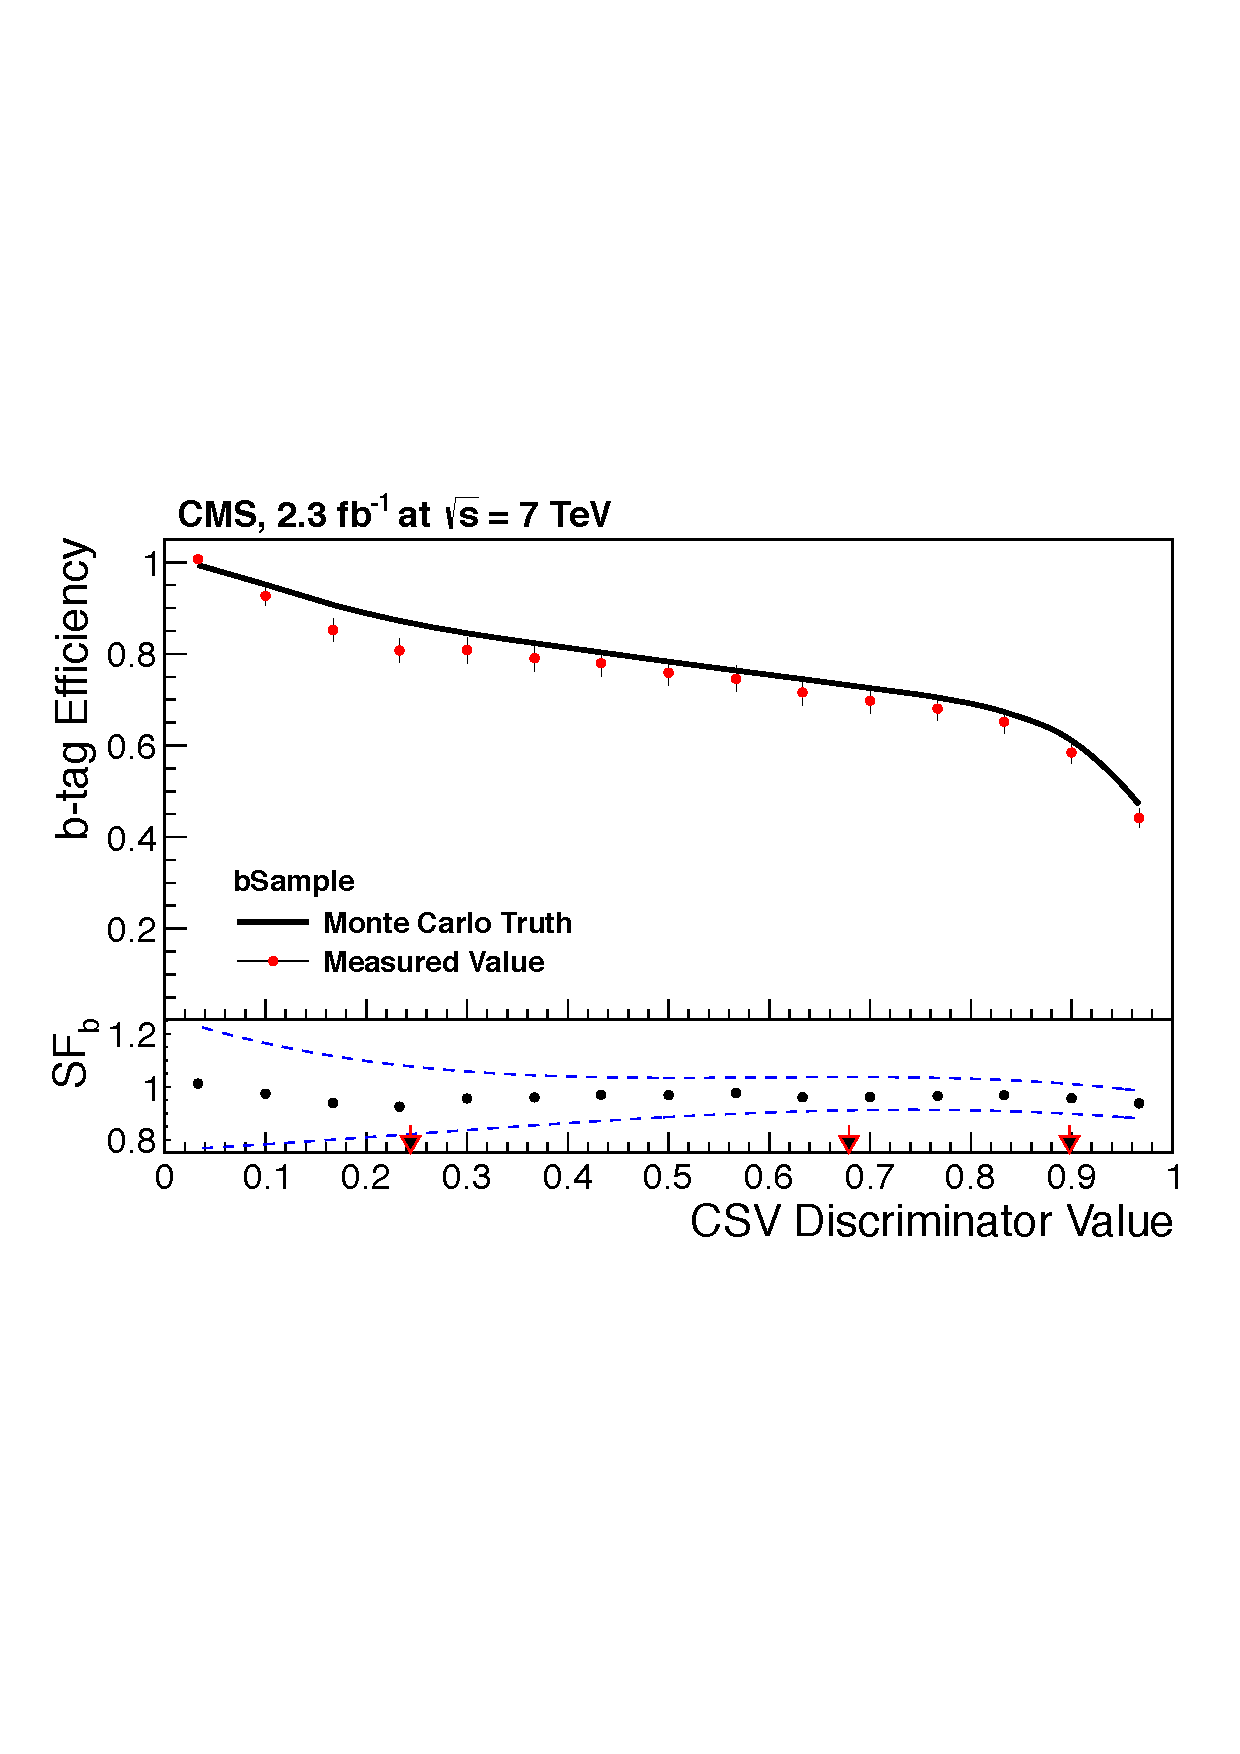
\includegraphics[width=0.7\columnwidth]{CSV_efficiency}
  \caption[b-tagging efficiency for the CSV algorithm]{Measured b-tagging efficiency as a function of the discriminator
  threshold for the CSV algorithm. The absolute b-tagging efficiency measured from data and predicted from simulation is
  shown in the upper histogram. The scale factors $\textrm{SF}_\textrm{b}$ are shown in the lower histogram, where the
  blue dashed lines represent the combined statistical and systematic uncertainty. The middle arrow indicates the
  ``medium'' working point used in the analyses \autocite{b-tagging_CMS}.}
  \label{fig:CSV_efficiency}
\end{figure}

\subsection{Missing transverse energy}
\label{ss:MET_reconstruction}
Due to momentum conservation, the sum of transverse momenta of all particles in the final state of proton-proton
collisions is expected to be zero. However, some particles can escape the detector without being reconstructed,
therefore creating the imbalance in transverse momentum which is referred to as missing transverse energy, defined as:
\begin{equation}
\label{eq:MET}
\METvec = - \sum_i \vec{p^i}_\mathrm{T}
\end{equation}
where $\vec{p^i}_\mathrm{T}$ are the transverse momentum vectors of all reconstructed particles. The modulus of
\METvec vector is denoted by \MET.

Accurate reconstruction of missing transverse energy is crucial for precise measurements of Standard Model processes
with neutrinos in the final state. Top quark pair semileptonic decay is one of such processes, therefore analyses
covered in this thesis implicitly (top mass) or explicitly (\ttbar cross section with respect to \MET-related variables)
rely on efficient reconstruction of \METvec. Misidentification and misreconstruction of any visible particles in the
event contribute to \METvec measurement, therefore it is a rather demanding task.

Just like in the case of leptons and jets, particle flow was used for \METvec reconstruction: in equation~\ref{eq:MET}
the transverse momentum vectors are of the particles reconstructed using the particle flow algorithm. This procedure
gives so-called raw \METvec on the output. The raw \METvec is systematically different from the true \METvec, which
denotes the transverse momentum carried by invisible particles. This happens mainly due to non-compensating nature of
the calorimeters, effects of pile-up, noise, etc. Therefore, a set of corrections is applied:
\begin{itemize}
 \item Type-0, which corrects \MET for pile-up;
 \item Type-I, a propagation of jet energy corrections (Section~\ref{sss:JEC}) to \MET;
 \item $xy$-shift correction, reducing the \METvec $\phi$ modulation.
\end{itemize}

The causes of systematic \METvec $\phi$ modulation include detector misalignment, beam spot displacement, inactive
calorimeter cells and anisotropic detector response. The $xy$-shift correction mitigates these effects, making the
measured \METvec distribution closer to the true \METvec distribution which is flat in $\phi$ because of the rotational
symmetry of the collisions.

All these corrections were applied to missing transverse energy in the analyses described in this work. However, the
$xy$-shift correction was not applied in the top mass analysis, since it was not available at the time. As this analysis
is not particularly sensitive to \MET, the $\phi$ modulation is not expected to affect the top mass measurement and its
resolution.

\section{Summary}
In this chapter, the Large Hadron Collider (LHC) has been introduced to the reader. The CMS experiment including all its
subsystems has been described in detail, the overview of the CMS computing model and analysis software have been shown.
Reconstruction and identification methods of various analysis objects including particle flow algorithm have been
discussed in detail.

% ------------------------------------------------------------------------

%%% Local Variables: 
%%% mode: latex
%%% TeX-master: "../thesis"
%%% End: 
